%%%%%%%%%%%%%%%%%%%%%%%%%%%%%%%%%%%%%%%%%%%%%
%                                           %
%  Karrera Bukaerako Proiekturako Plantilla %
%                                           %
%%%%%%%%%%%%%%%%%%%%%%%%%%%%%%%%%%%%%%%%%%%%%

%
% CONFIG: dokumentu estiloa definitu
%

\documentclass[a4paper,12pt,basque]{itsas_pfc}

%
% CONFIG: konfigurazio opzionala
%

%
% Erabilgarriak suerta dakizkizuken paketeak (gom = gomendatua, opz = opzionala)
%
\usepackage{fancyhdr}          % (gom)  goiburu eta oinak moldatzea ahalbidetzen du.
\usepackage{courier}           % (opz)  fuente hau erabili, defektuz.
\usepackage{setspace}          % (opz)  lerroen arteko espazioa aldatzea ahalbidetzen du.
\usepackage{longtable}         % (opz)  taulak orri bat baino gehiago luzatzea ahalbidetzen du.
\usepackage{lscape}            % (opz)  \landscape komanduaz zerbait apaisatua jartzea ahalbidetzen du.
\usepackage{color}             % (opz)  koloreri loturiko zenbait komandu (halaber \color).
\usepackage{rotating}          % (opz)  PSak eta EPSak biratzeko.
\usepackage{textcomp}          % (opz)  euro simboloa gehitzea ahalbidetzen du, \texteuro simboloaz.
\usepackage{minitoc}           % (opz)  kapitulu bakoitzean ToCak (gaien indizeak) gehitzea ahalbidetzen du.
\usepackage{epsf}              % (opz)  EPSen zenbait moldaketa ahalbidetzen du.
\usepackage[utf8x]{inputenc}   % (opz)  zenbait textu editorek karaktere gehiago (adbz. tildeak) erakustea ahalbidetzen du.
\usepackage[absolute]{textpos} % (gom)  textua nahi bezala orrian kokatzeko (portadarak beharrezkoa)
\usepackage{srcltx}            % (opz)  .dvi-tik .tex-era pasatzea ahalbidetzen du.
\usepackage[basque]{babel}     % (gom)  LaTeX euskarara moldatzeko.

%
% Marginak moldatzeko. Deskomentatu eta aldatu egiten ari zaren baldin badakizu.
% Ohar ematen diren baloreei pulgada bat gehitzen zaiola. Emandako baloreak A4
% papera eta itsas_pfc.cls estilorako aurredeterminatutakoak dira.
%
%\setlength{\oddsidemargin}{10pt}     % ezker margina orri ezpareetarako (ezkerra)
%\setlength{\evensidemargin}{52pt}    % ezker margina orri pareetarako (eskubia)
%\setlength{\textwidth}{390pt}        % textu gorputzaren zabalera

%
% Figuren kokapen automatikoa hobetzeko.
% (http://dcwww.camp.dtu.dk/~schiotz/comp/LatexTips/LatexTips.html#captfont-tik hartua)
%
\renewcommand{\topfraction}{0.85}
\renewcommand{\textfraction}{0.1}
\renewcommand{\floatpagefraction}{0.75}

%
% Orriaren goikaldea eta textua hasten deneko puntuaren arteko distantzia (hor doaz
% goiburuak). LaTeX kexatu egiten da 15pt baino txikiagoa denean.
%
\headheight 15pt

%
% Portadan erabiltzen den textpos paketearentzat.
%
\setlength{\TPHorizModule}{\paperwidth}
\setlength{\TPVertModule}{\paperheight}
\newcommand{\tb}[4]{\begin{textblock}{#1}[0.5,0.5](#2,#3)\begin{center}#4\end{center}\end{textblock}}

%
% Hemen zure komandoak defini ditzakezu.
% 
% \newcommand{cmd}[args]{def}
%
% cmd  = definitu nahi den komandoaren izena (adbz. \ura)
% args = argumentu kopurua
% def  = definizioa, non #1, #2... lehen, bigarren... argumentuekin trukatuko diren.
%
% Adibidez:
%
% \newcommand{\ura}[1]{H\ensuremath{_#1}O}
%
% "\ura{33}" idaztean, output-ean H33O aterako da (33 azpiindezea delarik).
%

%\newcommand{\zerbait}{zerbait}

%
% Hemen LaTeX-i esan diezaiokezu nondik moztu berak mozten ez dakizkien hitzak.
% Adibidez, "gnomonly" nola gidoiak (-) dauden lekutik mozteko:
%
\hyphenation{gno-mon-ly} 
 
%
% Hasieran orriak zenbaki erromatarrez zenba daitezela.
% Aurrerako zenbaki arabiarretara pasako gara.
%
\pagenumbering{Roman}


%
% Dokumentua berau hasten da
%

\begin{document}

%
% CONFIG: zenbait aldagairi balioa eman
%

%
% Fitxero honek LaTeX-en izen (aldagai) interno batzuk ditu, eta
% beraien balioa alda dezakezu. Adibidez, kapituluak "Sekzio" dei
% daitezela egin dezakezu.
%
\renewcommand\bibname{Bibliografia}                 % Bibliografia sekzioaren izena hori izan dadila.
\newcommand{\myname}{Josu López Fernández}                     % autorearen izena
\newcommand{\myboss}{Juan Antonio Pereira Varela}                     % gainbegiralearen izena
\newcommand{\thesistitle}{ASS formatuko azpititulu editorea Mac OS X sistemarako}             % lanaren izena
\newcommand{\worktype}{Karrera Bukaerako Proiektua} % lan mota
\newcommand{\logo}{Utils/ehu_logo.png}              % logoa duen fitxeroa (adbz. portadarako).
%\renewcommand{\tablename}{xxx}                     % taula azpiko izena (xxx 1: bla-bla-bla)
%\renewcommand{\figurename}{xxx}                    % figura azpiko izena (xxx 1: bla-bla-bla)
%\renewcommand{\listtablename}{yyy}                 % taulen indizearen izena.
%\renewcommand{\listfigurename}{yyy}                % figura indizearen izena.

% Nireak
\newcommand{\red}{\cellcolor[rgb]{1,0.8,0.8}}
\newcommand{\green}{\cellcolor[rgb]{0.8,1,0.8}}
\newcommand{\grey}{\cellcolor[rgb]{0.92,0.92,0.92}}
\newcommand{\bgrey}{\cellcolor[rgb]{0.8,0.8,0.8}}
\newcommand{\yellow}{\cellcolor[rgb]{1,0.93,0.8}}

%         
% EDUKINA: Portadaren edukina.
%         

%
% Fitxero honek KBP/Tesiaren lehenengo orria sortzen du, zeinak
% titulua, zure izena, gainbegiralearen izena etab. dituen.
%
% Horri honen gehiengoa, dena ezpada, komandoen bitartez gehitua dago, 
% (adbz. \thesistitle). Hauek Config/pfc_options.tex-en definituak izan dira.
%
% Editatu nahi den moduan.
%

\thispagestyle{empty} % orri honetan imprimatu ez zenbaki, ez goiburu, ez oinik

%
% Erabili \tb gauzak orrian kokatzeko. Erabilera:
%
% \tb{w}{h}{v}{t}
%
% non:
%
% w = textu kaxaren zabalera (1.0 = orri zabalera osoa)
% h = textu kaxaren posizio horizontala (0.0 = ezkerraldea, 1.0 = eskuinaldea)
% v = textu kaxaren posizio bertikala (0.0 goian, 1.0 behera)
% t = kaxan idatziko den textua
%

\tb{0.8}{0.50}{0.22}{\huge \thesistitle}                       % titulua
\tb{0.8}{0.50}{0.37}{\Large \worktype}                         % KBP edo Tesia ote den
\tb{0.5}{0.50}{0.40}{\today}                                   % sortze data (aldatu textu finkoaz)
\tb{0.8}{0.50}{0.45}{\large \myname}                           % autorearen izena
\tb{0.8}{0.50}{0.50}{\large \textit{Gainbegiralea:}\\ \myboss} % gainbegiralearen izena
\tb{0.9}{0.50}{0.90}{\includegraphics[width=0.30\columnwidth]{\logo}} % logo UPV/EHU

\ \clearpage                       % orria hemen bukatu
\thispagestyle{empty} \ \clearpage % orri txuria


%
% CONFIG: orriak 1 zenbakiaz kontatzen hasi.
%

% \cdpchapter erabili "eskubian" hasten diren ETA zenbakirik ez duten
% kapituluentzat (adbz. Eskertzak):
\newcommand{\cdpchapter}[1]{\cleardoublepage\chapter*{#1}}

% Hasi berriz batetik kontatzen orriak:
\setcounter{page}{1}


%
% EDUKINA: eskertzak/zitak/aitzinsolasa gehitu nahi izan ezkero.
%

%\cdpchapter{Eskertza}

Hau eskertza da.
 % eskertzak
%\cdpchapter{Aitzinsolasa}

Hau aitzinsolasa da.
          % aitzinsolasa

%
% CONFIG: Gaien Indizea (ToC).
% 

\dominitoc        % kapitulu bakoitzak bere ToC-a izan dezala ("minitoc" paketea behar du).
\tableofcontents  % ToC-a puntu honetan gehitu
\listoffigures    % Figura zerrenda (LoF) gehitu puntu honetan (opzionala).
\listoftables     % Taula zerrenda (LoT) gehitu puntu honetan (opzionala).

\cleardoublepage  % bukatu orria hemen.


%
% CONFIG: goiburu/oinaren estiloa definitzeko.
%

\pagestyle{fancy}                                % estilo hau aukeratu goiburu/oinentzat (gomendatua)
\fancyhf{}                                       % aurreko estiloa borratu (gero birdefinitzeko)
\fancyhead[LE,RO]{\textbf{\thepage}}             % Goiburua: orri zenbakia negritan.

\fancyhead[RE]{\nouppercase{\leftmark}}          % Goiburua: goi mailako informazioa (Kapitulua) eskubian (R) jarri,
                                                 % orri pareetan (E), dena maiuskulatan idatzi gabe (defektuzkoa
						 % litzatekena).

\fancyhead[LO]{\nouppercase{\rightmark}}         % Goiburua: behe mailako informazioa (Sekzioa) jarri, orri 
                                                 % ezpareetan (O), ezkerrean (L), dena maiuskulatan idazi gabe
						 % (defektuzkoa litzatekena).

\renewcommand{\headrulewidth}{0.5pt}             % Goiburua: azpimarratu goibura ("0pt" jarri kentzeko)
\renewcommand{\footrulewidth}{0pt}               % Oina: azpimarratu oina ("0pt" jarri kentzeko)


%
% CONTENT: Laburpena, balego.
%

\cdpchapter{Laburpena}

\thispagestyle{empty}

Gure helburua ASS (Advanced Substation Alpha) formatuko azpitituluei zuzendutako editorea egitea da. Formatu horretako fitxategiez gain, oso erabiliak diren SRT (SubRip) eta SUB (MicroDVD) formatuak editatu ahal izango dira, baita TXT fitxategiak inportatu ere. Lerroen eremu guztiak aldatzeko aukera egongo da, eskuz edo laguntzaileen bitartez, baita eremu batzuk multzoka editatzeko aukera ere.. Lerro bakoitzaren hasiera eta amaiera denborak aldatzeko, audio fitxategiak irekitzea eskeiniko du, modu grafikoz adieraziz honen anplitudea denboran zehar. Hauen formatua sistemak ireki dezakeen edozein izango da.

Honez gain, itzulpenerako laguntzaile bat edukiko du tresna bezala prozesu hau askartzeko beharrezkoa den informazioa soilik erakutsiz. Modu berdinean, pertsonaia desberdinen estiloak editatzeko tresna bat egongo da, baita estiloak aplikatzeko laguntzaile bat. Azkenik, ASS formatuak eskaintzen dituen karaokeak sortu eta editatu ahal izango dira, baita efektu konplexuagoak sortu aurrekoetatik abiatuz.

Guzti hau, Mac OS X sistema eragilerako garatuko da, aplikazioa natibo bezala. Horretarako, Objective-C 2.0 erabiliko da programazio lengoaia bezala, objektuei zuzendutako Cocoa API-a erabiliz. Erabiliko den lizentzia, GPLv2-a izango da.

\clearpage                         % orria bukatu
\thispagestyle{empty} \ \clearpage % orri txuria


%
% CONFIG: Kapituluen estiloa.
%

\setcounter{page}{1}    % Hasi berriz batetik kontatzen orriak
\pagenumbering{arabic}  % zenbaki arabeak erabili berriz orrientzat

% Ondo formateaturiko kapituluentzat, erabili \tocchapter,  
% \chapter ordez.
\newcommand{\tocchapter}[1]{\cleardoublepage\chapter{#1}\minitoc\newpage}


%
% EDUKINA: Honen ostean, gehitu nahi bezainbeste kapitulu/sekzio.
%

\tocchapter{Sarrera}

\section{Arazoa} % 1. Kapitulua: Sarrera
\tocchapter{Aurrekarien analisia}

\section{Sarrera}
Gaur egun badaude ASS formatuko azpitituluak editatzeko aplikazioak, gehienak Microsoft-en Windows sistema eragilerako eta batzuk Linux-erako. Mac OS X sistemarako ordea, ez dago erabilgarria den aplikaziorik.
\section{Azpititulu editoreak}
Atal honetan denboran zehar erabiliak izan diren azpititulu editoreak aztertu eta konparatuko ditugu.
\subsection{Sub Station Alpha}
Programa honek hasi zuen gure proiektuaren inguruko dena, programarekin batera, SSA formatua sortu zelako (honetatik atera zen gaur erabiltzen den ASS formatua). Microsoft Windows-erako doainiko programa pribatiboa da, 1996. urtean sortua britaniar baten eskutik, \textit{Kotus} ezizenarekin ezagutua. Ateratako azken bertsioa 2000. urtekoa da, beraz honen garapena duela asko bertan behera utzi zen.

Garatzailearen esanetan, programaren funtzioa azpitituluak modu erraz batean eta kalitate handiarekin sortzea zen, garaiko garestiak eta motelak ziren tresna komertzialen ordezko bat sortzea hain zuzen ere.

Nahiz eta bere garapena gaur egun kantzelatua egon, oraindik jende askok erabiltzen du, programa sinplea delako eta beraz oso erreza erabiltzeko, baita bere garaian erabiltzen zutenen ohituragatik.

Hiru fitxategirekin lan egiten du:
\begin{itemize}
\item SSA script-a.
\item Bideo fitxategi bat.
\item Audio fitxategi bat.
\end{itemize}

Azpitituluak editatzeko, SSA fitxategia da behar dugun bakarra, baina azpitituluak sinkronizatzeko audio fitxategia kargatu behar dugu. Fitxategi honen formatua \textit{PCM WAV} motakoa izan behar da, 8 bitekoa eta kanal bakarrekoa (\textit{mono}). Bideoaren erabilera erreferentzia bat edukitzeko mugatzen da, azpitituluak ez dituelako erakusten prozesatu ondoren ikusiko diren bezala.
\begin{figure}[htb]
\begin{center}
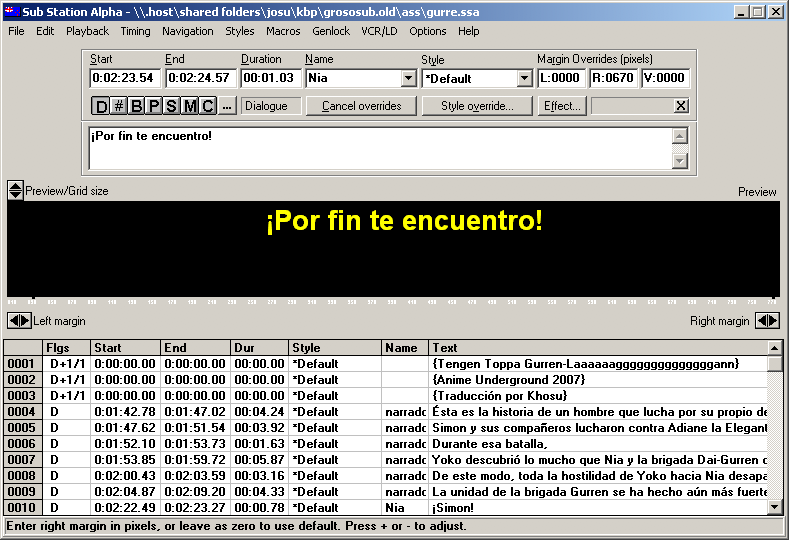
\includegraphics[width=\columnwidth, natwidth=789pt, natheight=540pt]{Pictures/Chapter2/ssa-script.png}
\caption{Sub Station Alpha azpititulu fitxategi batekin}
\label{ssa-script}
\end{center}
\end{figure}

\ref{ssa-script}~Irudian ikusten dugun bezala programak informazioa guztia lehio berdinean erakusten du. Nahiz eta erabilgarria izan, oso astuna suertatzen da beste programekin konparatuz. Aipatzekoa da programarekin lanean gabiltzanean zenbait \textit{bug}-en ondorioz programaren funtzionamendua zuzena ez dela.

Aldaketak ez dira azpiko taulan egiten, goiko partean baizik, non aukeratua dugun lerroaren informazioa guztia eskuragarri dugun.

Aurrebista ez da batere zehatza, aukeratutako lerroa erakusten du bere letra-mota eta kolorearekin atzekalde beltzean soilik. Beraz, ez digu erakusten adibidez itzalaren kolorea, azpitituluaren posizioa pantailan, etab. Ikusten dugunez, aurrebista honek ez du funtzionalitate handirik.
\begin{figure}[htb]
\begin{center}
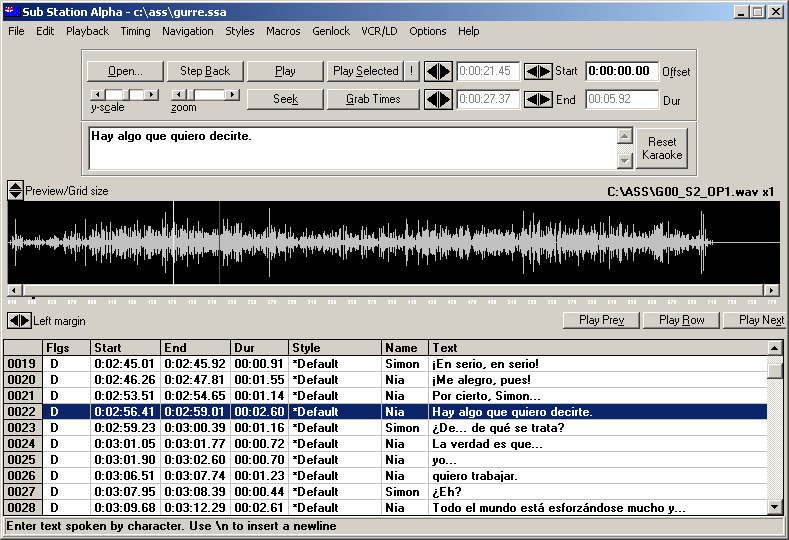
\includegraphics[width=\columnwidth, natwidth=789pt, natheight=540pt]{Pictures/Chapter2/ssa-audio.png}
\caption{Sub Station Alpha audio fitxategi batekin}
\label{ssa-audio}
\end{center}
\end{figure}

Azpitituluez gain audio fitxategi bat kargatzerakoan, \ref{ssa-audio}~Irudian ikusten dugunarekin topatuko gara. Azpitituluen aurrebistaren ordez, audioaren uhin-forma erakusten digu. Lerro baten hasiera eta bukaera denborak esleituko ditugu hemen saguaren bidez click eginez nahi dugun lekuan. Lehen aipatu dugun bezala, audioaren formatua ezin daiteke edozein izan, \textit{PCM WAV} formatuan egon behar da, 8 bitekoa eta kanal bakarrekoa, beraz ez da oso ondo entzuten MP3 edo OGG Vorbis-ekin alderatuz, nahiz eta formatu hauek konprimituak izan, kalitate askoz hobeagoa eskaintzen dutelako.

Ondorio bezala, Sub Station Alpha erabilgarria da, baina gaur egungo berriagoak diren aukerak erabiltzea gomendagarria da, erosoagoak direlako.

\subsection{Medusa}
2002. urtean, \textit{Sub Station Alpha}-ren garapena 2 urtez geldirik egon ondoren, editore hau kaleratu zuen programatzaile italiar batek, \textit{Kaidousama} ezizenarekin ezagutua. Urte honetarako, SSA formatuaren eboluzioa atera zen, \textit{Advanced Substation Alpha} (ASS), gaur egun erabiltzen dena hain zuzen. Aurreko programa bezala, hau ere Microsoft-en Windows sistema eragilerako garatu zen Visual Basic 6 erabiliz.

Aldaketa handiak suposatu zituen editore honek, gehienbat ASS formatuaren inplementazioagatik. Hauek dira aipagarrienak:
\begin{itemize}
\item SSA ordez ASS da bere formatu natiboa.
\item Audio formatu gehiago erabili ditzake, adibidez \textit{MP3} edo \textit{OGG Vorbis}.
\item Bideo bidezko sinkronizazioa.
\item ASS komandoen sintaxiaren nabarmendua.
\item Karaokeak silaba bidez sinkonizatzeko aukera, azkarra eta erosoa.
\end{itemize}

Hala ere, lan egiteko modua bere aintzindariaren antzekoa da, horregatik lortu zuen \textit{Sub Station Alpha} erabiltzen zuten askok hau erabiltzea.
\begin{figure}[htb]
\begin{center}
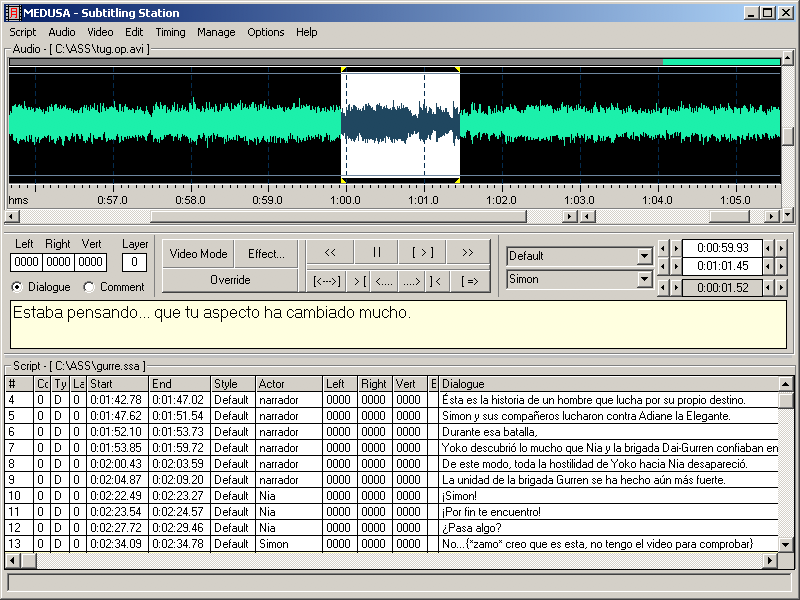
\includegraphics[width=\columnwidth, natwidth=800pt, natheight=600pt]{Pictures/Chapter2/medusa-audio.png}
\caption{Medusa editorea azpititulu eta audio fitxategi batekin}
\label{medusa-audio}
\end{center}
\end{figure}

\ref{medusa-audio}~Irudian ikusten dugunez, nahiz eta antzeko interfazea izan, askoz atseginagoagoa da bisualki, baita bere erabileran ere.

Funtzionalitate berriak sartu zituen, adibidez, aukeratutako audio zatia erreproduzitzeaz gain, honen testuingurua (aurreko eta ondorengo 500 milisegunduak), aukeratutakoaren hasiera, amaiera, etab. erreproduzitzeko aukera ematen du. Honez gain, ASS formatuarekin lan egiten duenez, estilo mota berriak onartzen ditu. Azpitituluen aurrebista ere badu, VSFilter erabiliz.
\begin{figure}[htb]
\begin{center}
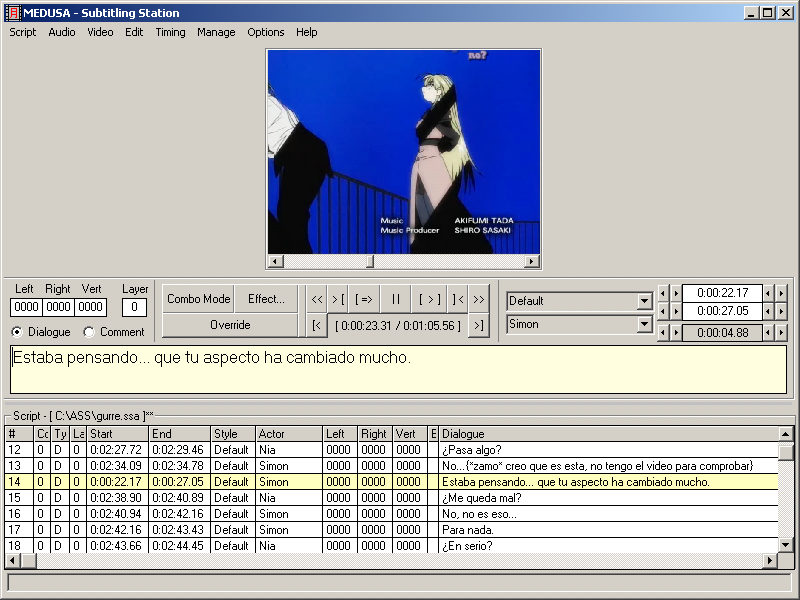
\includegraphics[width=\columnwidth, natwidth=800pt, natheight=600pt]{Pictures/Chapter2/medusa-bideo.png}
\caption{Medusa editorea azpititulu eta bideo fitxategi batekin}
\label{medusa-bideo}
\end{center}
\end{figure}

Bideo fitxategi bat kargatzerakoan, \ref{medusa-bideo}~Irudian ikusten dena bistaratuko da. Azpitituluak sinkronizatzeko erabili dezakegu hau, baita hauek ikusteko ere. Dena den, alde txar bat dauka: \textit{DirectShow}\footnote{Microsoft Windows-en erabiltzen den multimedia API-a} erabiltzen du, beraz erakusten dituen \textit{frame}-ak ez dira zehaztasun handiarekin benetakoak. Ondorioz, bideoaren frame batean jarritako azpititulu bat, probabilitate handiarekin beste frame batean agertuko da gero bideoan. Ikusten dugunez, nahiz eta \textit{Sub Station Alpha}-rekin konparatuz bideoarekin hobeto lan egin daitekeen, ez da oso erabilgarria.

\textit{Medusa}-k momentuan ekarri zuen funtzionalitate hoberena karaokeak sinkronizatzeko interfazea izan zen, \ref{medusa-karaoke}~Irudian ikusten duguna hain zuzen.
\begin{figure}[htb]
\begin{center}
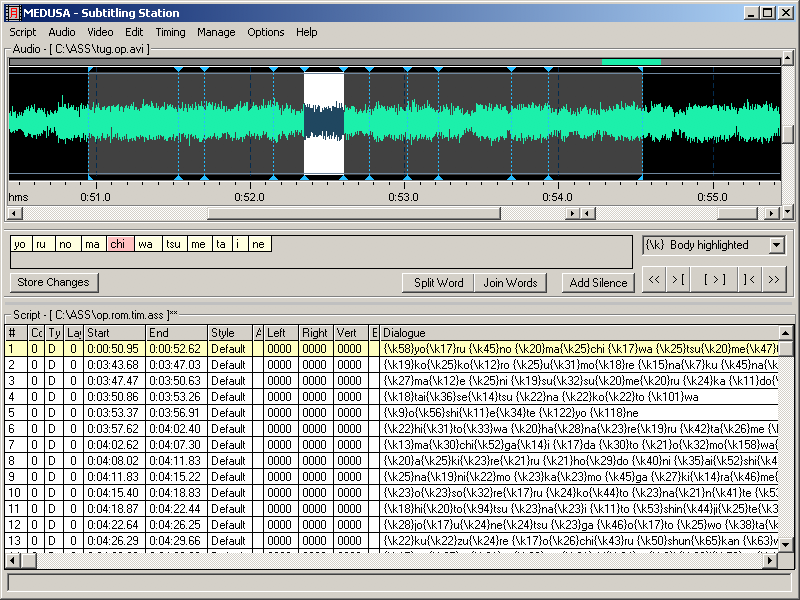
\includegraphics[width=\columnwidth, natwidth=800pt, natheight=600pt]{Pictures/Chapter2/medusa-karaoke.png}
\caption{Medusa editorearen karaokeak sinkronizatzeko interfazea}
\label{medusa-karaoke}
\end{center}
\end{figure}

Ikusten dugunez, silabaka banatzen da lerroko testua, eta hauek batu edo banatu eta isiluneak gehitu ahal ditzakegu. Gainera, silaba baten hasiera edo bukaera denbora aldatzean, bere ondokoak ere aldatzen dira (adibidez amaiera denbora murriztean, hurrengo silabaren hasiera denbora lehenago izango da). \textit{Sub Station Alpha}-rekin alderatuz, izugarrizko aurrerapena zen, honetan eskuz egin behar zirelako inolako laguntzarik gabe. Minutu t'erdiko abestiaren karaokea egitea \textit{Sub Station Alpha}-rekin ordu pare bateko esfortzua eskatzen zuen, \textit{Medusa}-rekin karaoke bera egitea 30 minutu inguru, hau da, laurden bat.

Ondorioz, nahiz eta bere aurrekaria baino programa hobeagoa izan, zenbait akats ditu. Adibidez, nahiz eta MP3-rekin lan egin ahal izan, hau kargatzerakoan PCM formatura pasatzen du, 16 bitekoa, \textit{estereo} eta 44 KHz-tako maiztasunarekin, eta disko gogorrean gordetzen du. 24 minutuko MP3 batek gutxi gora behera 30 MB-eko tamaina du, baina PCM-ra pasatzerakoan 300 MB-eko fitxategi bat lortuko dugu.

2004. urtean bere garapena bertan behera utzi zen, egileak Delphi-n birprogramatzea erabaki zuelako (\textit{ChronoSub} izenarekin), baina ez da berririk egon honen inguruan.

\subsection{Aegisub}
Hau da egungo ASS formatuko azpititulu editorerik hoberena. Azpititulatzaile komunitateak berak garatu du, \textit{Sub Station Alpha}-k eta \textit{Medusa}-k zituzten arazoak konpontzeko asmoarekin.

Hasieran \textit{Visual SSA} izenarekin ezagutu zen, ondoren \textit{Visual ASS} bezala eta azkenik \textit{Aegisub} izenarekin geratu da. 2005. urtean agertu zen v1.00 \textit{beta} bertsioa, eta 1.07 bertsiotik aurrera bere kodea askatu zuten BSD\footnote{\url{http://en.wikipedia.org/wiki/BSD_license}} lizentzia batekin. Bere denbora librea azpititulatzen pasatzen zuten bi programatzailek hasi zuten proiektua, baina gaur egun jende asko dago garapen taldean, horregatik gaur egun dagoen aplikaziorik erabilena eta konpletuena da.

C++ lengoiaz garatuta dago, eta nahiz eta hasieran Windows-erako bakarrik izan, gaur egun Linux-en funtzionatzen du, baita Mac OS X-en ere (garatzaileen esanetan, baina honen inguruan aurrerago hitz egingo dugu).

Hauek dira programak dituen ezaugarri nagusiak:
\begin{itemize}
\item ASS formatuaren erabilera natiboa, honez gain SSA, SRT eta TXT formatuak inportatu ditzake.
\item Unicode testu kodifikazioan dauden fitxategiak erabil ditzake (oso erabilgarria beste hizkuntzetako karaktereak sartzeko).
\item Karaokeak modu automatizatuan egiteko aukera \textit{Lua} programazio lengoaia erabiliz.
\item Sintaxiaren nabarmendua.
\item Bideoak ireki ditzake \textit{AviSynth} erabiliz.
\item Azpitituluak erakusten ditu \textit{VSFilter} erabiliz, beraz prozesatu ondoren ikusiko diren bezala.
\item \textit{DirectShow}-k dekodifikatu dezakeen edozein audio fitxategirekin lan egiteko ahalmena.
\item Karaokeen sinkronizazioarako sistema aurreratua.
\item Itzulpen prozesurako laguntzaile bat.
\item Estiloak gorde daitezke script desberdinetan erabili ahal izateko.
\item Estiloak aplikatzeko laguntzailea bat.
\item Azpitituluen arteko talkak antzematen ditu.
\item Makroen erabilera zenbait ataza egiteko.
\item Azpitituluak modu grafikoan editatzeko aukera.
\end{itemize}

Bere atzean dagoen garapen taldeari esker, funtzionalitate asko eta onak ditu programa honek.

\begin{figure}[htbp]
\begin{center}
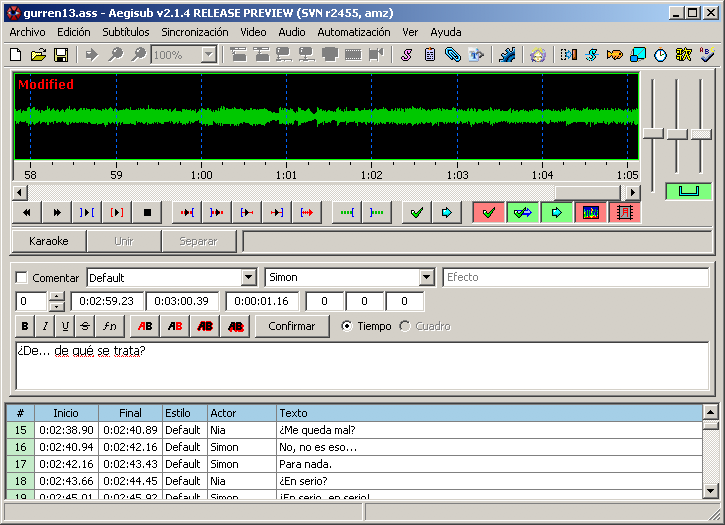
\includegraphics[width=\columnwidth, natwidth=725pt, natheight=525pt]{Pictures/Chapter2/aegisub-audio.png}
\caption{Aegisub editorea azpititulu eta audio fitxategi batekin}
\label{aegisub-audio}
\end{center}
\end{figure}

\ref{aegisub-audio}~Irudian ikus dezakegunez, interfazea antzekoa da \textit{Sub Station Alpha} eta \textit{Medusa}-rekin konparatuz, baina hauek baino erosoagoa da lan egiteko orduan, dauzkan aukera mordoagatik.

Audio bidezko sinkronizazioarako, erabili nahi ditugun teklak definitu ditzakegu, horrela aurreko bi programetan bezala lan egin ahal izateko. Audioa oso azkar kargatzen da programan eta ez ditu aldi baterako fitxategi handiak erabiltzen. Honen ordez, ahal duen guztia kargatzen du RAM memorian modu azkar batean atzitu ahal izateko. Uhin-forma marrazteko funtzioa baita ere azkarra da, eta hau asko eskertzen da sinkronizatzerakoan, asko mugitzen baikara uhin-formaren ikuspegitik zehar. Honez gain, uhin-espektroa marraztu dezake \textit{FFT}\footnote{\url{http://en.wikipedia.org/wiki/Fast_Fourier_transform}} erabiliz. Hau oso erabilgarria da espektroan gizakion ahotsa modu errazean ikus dezakegulako. \ref{aegisub-spectrum}~Irudian agertzen da Aegisub-ek nola erakusten duen audio modu honetan.
\begin{figure}[htbp]
\begin{center}
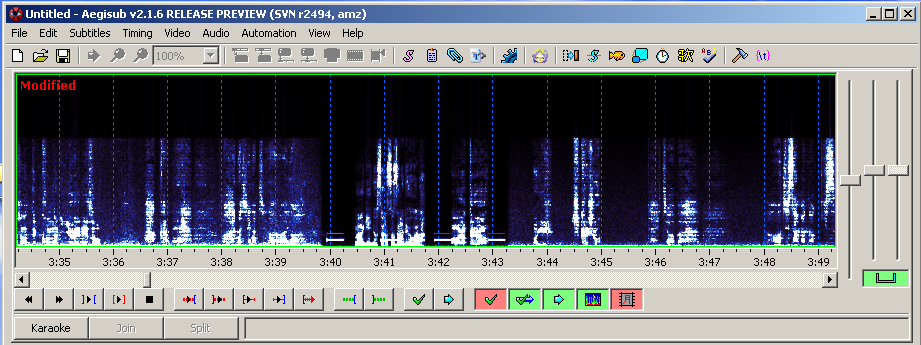
\includegraphics[width=\columnwidth, natwidth=728pt, natheight=532pt]{Pictures/Chapter2/aegisub-spectrum.png}
\caption{Aegisub-en audioaren espektroa}
\label{aegisub-bideo}
\end{center}
\end{figure}

Bideoa kargatzeaz eta ikusteaz gain, bere gainean lan egin dezakegu. Testua mugitu, biratu (hiru ardatzekiko), tamainaz aldatu, \textit{clip}-ak egin, etab. saguarekin modu erraz eta ikusgarri batean. Guzti hau ikus dezakegu \ref{aegisub-bideo}~Irudian (ezkerraldean daude testuan aldaketak egiteko tresnak).

\begin{figure}[htbp]
\begin{center}
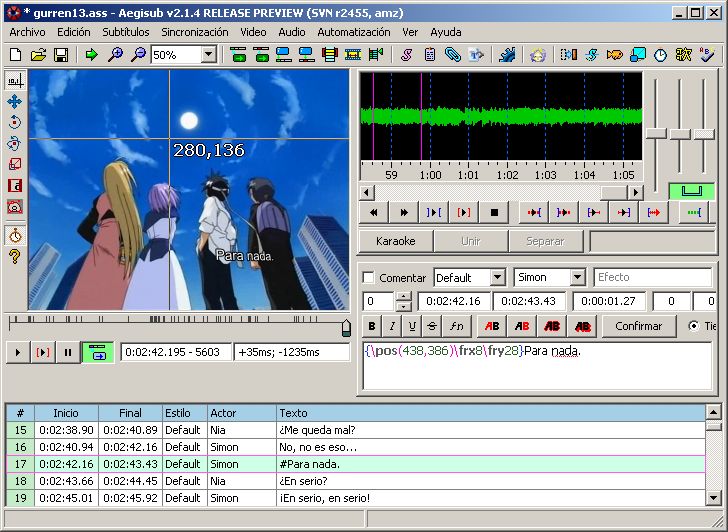
\includegraphics[width=\columnwidth, natwidth=728pt, natheight=532pt]{Pictures/Chapter2/aegisub-bideo.png}
\caption{Aegisub editorea azpititulu eta bideo fitxategi batekin}
\label{aegisub-bideo}
\end{center}
\end{figure}

Bestalde, post-prozesaketa aukerak eskeintzen ditu lehenengo aldiz mota honetako programetan, oso erabilgarriak diren ekintzak egin ahal izateko. Adibidez, tarte batean hurbil dauden azpitituluak modu jarraian ipiniko ditu, horrela hutsunerik utzi gabe testu bat eta bestearen artean, edo lerro bat bestearen gainean ez egoteko momentu batez. Beste adibide bat: azpitituluen denborak \textit{keyframe}\footnote{\url{http://en.wikipedia.org/wiki/Key_frame}} batetik hurbil badaude, honetara egokituko ditu. Guzti honetarako \ref{aegisub-post}~Irudian dagoen lehioa erabitzen da.

\begin{figure}[htbp]
\begin{center}
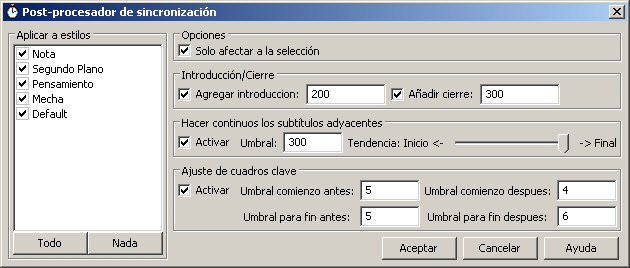
\includegraphics[width=\columnwidth, natwidth=630pt, natheight=268pt]{Pictures/Chapter2/aegisub-post.png}
\caption{Aegisub editorearen post-prozesaketa aukerak}
\label{aegisub-post}
\end{center}
\end{figure}

\begin{figure}[htp]
\begin{center}
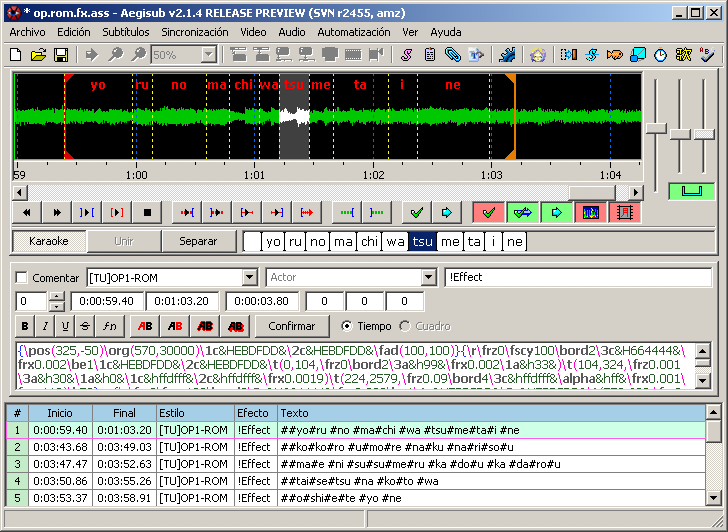
\includegraphics[width=\columnwidth, natwidth=728pt, natheight=532pt]{Pictures/Chapter2/aegisub-karaoke.png}
\caption{Aegisub editorearen karaokeak sinkronizatzeko interfazea}
\label{aegisub-karaoke}
\end{center}
\end{figure}

Azkenik, karaokeak egiteko \textit{Medusa}-k daukan sistemaren antzeko bat dauka \ref{aegisub-karaoke}~Irudian ikus dezakegun bezala, oso erosoa eta azkarra lan neketsu hau egiteko.

Honez gain, karaokeen gainean efektuak, aplika ditzakegu karaoke konplexuago eta politagoak egin ahal izateko, \textit{Lua}\footnote{\url{http://www.lua.org/}} \textit{scripting} lengoaiaren bidez. Hau existitu baino lehenago, kalkulu guztiak kalkulagailu bidez egiten ziren, lan oso neketsua eta motela izanik. Gainera, sortzen ditugun efektuak momentuan ikus ditzakegu horrela lan fluxua azkartuz.

Aurreko guztia kontuan hartuz, ondoriozta dezakegu hau dela gaur egun dagoen azpititulu editorerik hoberena eskeintzen duen guztiagatik eta kalitateagatik. Lehen esan bezala, suposatzen da Mac OS X-en funtzionatzen duela, eta horrela da, konpilatu eta exekuta dezakegu, baina funtzionalitate gehienetan akatsak ditu, adibidez, audio fitxategi bat kargatzerakoan erroreak agertuko zaizkigu eta ezingo dugu audioarekin lan egin. Gainera noizbehinka aplikazioa itxi egiten da guk ezer arrarorik egin gabe, beraz ondoriozta dezakegu ez dela batere erabilgarria Mac OS X sisteman.

\section{Konparaketa}
\ref{konparaketa}~taulan daude hiru programa hauen ezaugarriak. Bertan ikus dezakegunez, Aegisub da hiruretatik hoberena.
\begin{longtable}{|l|c|c|c|}
\hline
& \grey Sub Station Alpha & \grey Medusa & \grey Aegisub\\
\hline
\endhead
\hline
\caption{\label{konparaketa}Aztertutako programen ezaugarriak}
\endfoot
\grey Bertsioa & 4.08 & 0.1.2.0 & 2.00alpha\\
\hline
\grey Garapena & \red Bertan behera & \red Bertan behera & \green Aktiboa\\
\hline
\grey Lizentzia & \red Itxia & \red Itxia & \green BSD\\
\hline
\grey Lengoaia & Visual Basic & Visual Basic & C++\\
\hline
\multicolumn{4}{|l|}{\bgrey \textbf{Azpititulu formatuak}}\\
\hline
\grey SSA & \green Bai(natiboa) & \green Bai & \green Bai\\
\hline
\grey ASS & \red Ez & \green Bai(natiboa) & \green Bai(natiboa)\\
\hline
\grey SRT & \red Ez & \green Bai & \green Bai\\
\hline
\grey Testu planoa & \green Bai & \green Bai & \green Bai\\
\hline
\multicolumn{4}{|l|}{\bgrey \textbf{Karaktere kodifikazioa}}\\
\hline
\grey Lokala & \green Bai(natiboa) & \green Bai(natiboa) & \green Bai\\
\hline
\grey Unicode & \red Ez & \red Ez & \green Bai(natiboa)\\
\hline
\grey Autodetekzioa & \red Ez & \red Ez & \green Bai\\
\hline
\multicolumn{4}{|l|}{\bgrey \textbf{Sistema eragileak}}\\
\hline
\grey Microsoft Windows & \green Bai & \green Bai & \green Bai\\
\hline
\grey Linux & \red Ez & \red Ez & \yellow Osatugabea\\
\hline
\grey Mac OS X & \red Ez & \red Ez & \red Erabilezina\\
\hline
\multicolumn{4}{|l|}{\bgrey \textbf{Audioa}}\\
\hline
\grey PCM WAV & \yellow 8 bit mono & \green Bai & \green Bai\\
\hline
\grey MP3 & \red Ez & \green Bai & \green Bai\\
\hline
\grey Ogg Vorbis & \red Ez & \green Bai & \green Bai\\
\hline
\grey AAC & \red Ez & \red Ez & \green Bai\\
\hline
\grey AC3 & \red Ez & \red Ez & \green Bai\\
\hline
\grey Bideotik & \green Bai & \red Ez & \green Bai\\
\hline
\grey Uhin-forma & \green Bai & \green Bai & \green Bai\\
\hline
\grey Espektroa & \red Ez & \red Ez & \green Bai\\
\hline
\multicolumn{4}{|l|}{\bgrey \textbf{\textit{Typesetting}}}\\
\hline
\grey Bisualki & \red Ez & \red Ez & \green Bai\\
\hline
\grey Estilo editorea & \green Bai & \green Bai & \green Bai\\
\hline
\grey Estilo kudeatzailea & \green Bai & \green Bai & \green Bai\\
\hline
\grey Estilo aurrebista & \green Bai & \red Ez & \green Bai\\
\hline
\multicolumn{4}{|l|}{\bgrey \textbf{Audio sinkronizazioa}}\\
\hline
\grey Elkarrizketak & \green Bai & \green Bai & \green Bai\\
\hline
\grey Karaokeak & \yellow Sinplea & \green Bai & \green Bai\\
\hline
\multicolumn{4}{|l|}{\bgrey \textbf{Azpitituluen gaineko eragiketak}}\\
\hline
\grey Shift, Split eta Join & \green Bai & \green Bai & \green Bai\\
\hline
\grey Bikoiztu & \red Ez & \red Ez & \green Bai\\
\hline
\grey Undo/Redo & \red Ez & \red Ez & \green Bai\\
\hline
\grey Sintaxi nabarmendua & \red Ez & \green Bai & \green Bai\\
\hline
\grey Regex & \red Ez & \red Ez & \green Bai\\
\hline
\multicolumn{4}{|l|}{\bgrey \textbf{Tresnak}}\\
\hline
\grey Itzulpen laguntzailea & \red Ez & \red Ez & \green Bai\\
\hline
\grey Zuzentzailea & \green Bai & \red Ez & \green Bai\\
\hline
\grey Karaoke efektuak & \red Ez & \yellow Sinplea & \green Bai\\
\hline
\multicolumn{4}{|l|}{\bgrey \textbf{Bestelakoak}}\\
\hline
\grey Automatikoki gorde & \green Bai & \red Ez & \green Bai\\
\hline
\grey Segurtasun kopiak & \red Ez & \red Ez & \green Bai\\
\hline
\grey Dokumentu anitz irekita & \red Ez & \red Ez & \red Ez\\
\end{longtable}

\section{Ondorioak}

Kapitulu honetan aztertu dugunez, aplikazio bat dago azpititulugintzako lehengo postuan, \textit{Aegisub} hain zuzen ere. Nahiz eta garatzaileen esanetan Mac OS X-en funtzionatu, ez da batere erabilgarria. Konpilatu eta exekutatu dezakegu, baina adibidez ezin dugu audiorik kargatu eta honekin lan egin, beraz, programaren funtzionalitatea asko murrizten da.

\textit{Aegisub}-ek lizentzia irekia du, BSD lizentzia hain zuzen ere, beraz, zergatik ez dugu eraldatu eta guri interesatzen zaigun plataformarako egokitu? \textit{Aegisub} C++ lengoaian dago idatzita eta wxWidgets\footnote{\url{http://www.wxwidgets.org/}}-ekin dago programatuta. Honen ondorioz, programa ez dago sisteman integratua, ez dauka beste aplikazio guztien itxura berdina, beraz nahiz eta bere funtzionamendua egokia izan aplikazio arrotza izango da sistemako beste guztiekin konparatuta. Mac OS X-eko aplikazioa natiboak ordez, Objective-C\footnote{\url{http://en.wikipedia.org/wiki/Objective-C}} lengoaian daude idatzita. Objektuei zuzendutako lengoaia da, C lengoaiaren gainean eraikia, honi Smalltalk\footnote{\url{http://en.wikipedia.org/wiki/Smalltalk}}-eko mezuak gehituz. Aplikazio grafikoak egiteko, Cocoa\footnote{\url{http://developer.apple.com/cocoa/}} API-a erabiltzen da.

Dena den, \textit{Aegisub}-ek funtzionalitate asko dauzka, eta proiektu honetan, garapen denbora kontuan edukita ezin izango dugu hain programa konplexua egin, beraz funtzionalitate bakar batzuk inplementatuko dira.
 % 2. Kapitulua: Aurrekarien analisia
\tocchapter{Proiektuaren helburu dokumentua}

\section{Deskribapena}
Garatuko den aplikazioa azpititulu editore bat izango da, Mac OS X sistema eragilerako. Azpititulu berriak sortu edo sortuta daudenak editatu ahal izango ditu, formatu erabilienetan: ASS, SRT eta SUB. TXT fitxategiak ere inportatu ahal izango ditu azpitituluen sorrerarako.

\section{Helburua}
Helburu nagusia aplikazioaren garapena da, horretarako hainbat zelai ikutzen direlarik: fitxategien maneiua, audio fitxategien erabilera (audioa marrazteko eta erreproduzitzeko), karaokeen sorkuntza, etab.
Aplikazioaren atal gehienak programatu beharko dira, nahiz eta agian zenbait software edo liburutegi erabiliko diren gure aplikazioak behar duen funtzionalitate bat eskaintzen badute.
Proiektua lizentzia aske baten menpe garatuko da, \textbf{GNU GPVv2} hain zuzen ere, honako arrazoiengatik:
\begin{itemize}
\item Edonork aplikazioa mugarik gabe erabili ahal izatea.
\item Proiektua amaitzean, norbaitek jarraitu nahi badu ia arazorik gabe egin ahal izatea (lizentzia berdinarekin).
\item Aplikazioaren kalitatea hobetzea (jende gehiagok erabili/garatu).
\end{itemize}
Beste helburu bat, proiektu \textit{handi} baten garapenak suposatzen duena ulertzea eta dokumentatzea da.
Azkenik, proiektuen garapenarekin zerikusia duten tresnak erabiliko dira: bertsioen kontrol sistema (Subversion), bug-en gestio sistema, etab. Honetarako, Assembla.com webguneak dohainik eskaintzen dituen baliabideak erabiliko dira. Bertan proiekturako \textit{space} bat sortuko da eta honako zerbitzuak erabili ahal izango ditugu: foroak, wikiak, ticket-ak, Subversion bertsioen kontrol sistema bezala, fitxategiak igotzeko aukera, etab.

\section{Norainokoa}
Hauek dira egin beharrekoak:
\begin{enumerate}
\item Aplikazioaren garapena:
	\begin{itemize}
	\item Formatu desberdinekin lan egitea (ASS, SRT eta SUB).
	\item Audioa ireki ahal izatea hau marrazteko eta erreproduzitzeko.
	\item Zenbait laguntzaileren sorrera (itzulpenerako, karaokeak sortzeko, etab.).
	\end{itemize}
\item Aplikazioa sistemarekin ondo integratzea.
\item Erabiltzailearentzako erabilpen gidak sortzea, hau da, programaren funtzionalitateak dokumentatzea.
\item Instalatzeko erraza den pakete bat sortzea, erabiltzaileak programa konpilatu behar ez izateko.
\end{enumerate}

\subsection{Lanaren dekonposaketa egitura diagrama}
\begin{figure}[htb]
\begin{center}
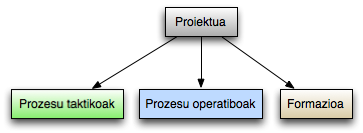
\includegraphics[width=\columnwidth, natwidth=817pt, natheight=349pt]{Pictures/Chapter3/LDE.png}
\caption{Lanaren dekonposaketa egitura diagrama}
\label{lde}
\end{center}
\end{figure}

\subsection{Azpiatazen zerrenda}
\begin{itemize}
\item \textbf{Kudeaketa:}
	\begin{itemize}
	\item K1 - Bilerak:
		\begin{itemize}
		\item K11 - Ohiko bilerak.
		\item K12 - Aurrerapen bilerak:
			\begin{itemize}
			\item K121 - Bilera burutu.
			\item K122 - Egoera txostena egin.
			\end{itemize} 
		\end{itemize}
	\item K2 - Artxiboaren kudeaketa.
	\end{itemize}
\item \textbf{Planifikazioa:}
	\begin{itemize}
	\item P1 - Proiektuaren helburu dokumentua egin.
	\item P2 - Iterazio berriaren planifikazioa.
	\end{itemize}
\item \textbf{Garapena:}
	\begin{itemize}
	\item G1 - Eskakizunen bilketa:
		\begin{itemize}
		\item G11 - Erabilpen kausen eredua egin.
		\item G12 - Domeinuaren eredua egin.
		\item G13 - Interfazearen prototipoa egin.
		\end{itemize}
	\item G2 - Analisia:
		\begin{itemize}
		\item G21 - Sistemako sekuentzia diagramak egin.
		\item G22 - Kontratuak egin.
		\end{itemize}
	\item G3 - Diseinua:
		\begin{itemize}
		\item G31 - Sekuentzia diagramak egin.
		\item G32 - Klase diagrama egin.
		\item G33 - Probak diseinatu.
		\end{itemize}
	\item G4 - Inplementazioa.
	\item G5 - Probak egin.
	\end{itemize}
\item \textbf{Dokumentazioa:}
	\begin{itemize}
	\item D1 - Eskuliburua egin.
	\item D2 - Memoria egin.
	\end{itemize}
\item \textbf{Bukatzea:}
	\begin{itemize}
	\item B1 - Defentsa:
		\begin{itemize}
		\item B11 - Edukiak aukeratu.
		\item B12 - Aurkezpena prestatu.
		\item B13 - Aurkezpena egin.
		\end{itemize}
	\end{itemize}
\item \textbf{Formazioa:}
	\begin{itemize}
	\item F1 - Aurrekarien analisia:
		\begin{itemize}
		\item F12 - Azpititulu editoreen bilaketa.
		\item F13 - Aukeratutako editoreen analisia.
		\item F14 - Konparaketa eta ondorioak.
		\end{itemize}
	\item F2 - Objective-C ikastea.
	\item F3 - Cocoa ikastea.
	\end{itemize}
\end{itemize}

\subsection{Emangarrien zerrenda}
\begin{longtable}{|p{70px}|p{250px}|p{30px}|}
\hline
\grey \textbf{Emangarria} & \grey \textbf{Deskribapena} & \grey \textbf{Ataza}\\
\hline
\endhead
\hline
\caption{\label{emangarriak}Sortuko diren emangarriak}
\endfoot
\textit{Akta} & Bilera bakoitzean tratazen diren gaien laburpena & K11\\
\hline
\textit{Egoera txostena} & Proiektuaren faseen egoera aztertzen duen dokumentua & K122\\
\hline
\textit{PHD} & Proiektua planifikatzeko hasierako unean sortutako dokumentu aldaezina & P1\\
\hline
\textit{LDE diagrama} & Ataza eta azpiataza garrantzitsuenak adierazten dituen diagrama & P1\\
\hline
\textit{Gantt diagrama} & Planifikatutako ekintzen egutegiaren adierazpide grafikoa, non ekintza bakoitzaren iraupena adierazten den & P1\\
\hline
\textit{Erabilpen kasuen eredua} & Programaren portaera adierazten duen diagrama & G11\\
\hline
\textit{Domeinuaren eredua} & Domeinuan agertzen diren objektuen atributuak eta erlazioak adierazten dituen diagrama & G12\\
\hline
\textit{Interfazearen prototipoa} & Interfazea nolakoa izango den & G13\\
\hline
\textit{Sistemako sekuentzia diagramak} & Erabilpen kasu bakoitzaren portaera adierazten duten diagramak & G21\\
\hline
\textit{Kontratuak} & Eragiketen espezifikazioa & G22\\
\hline
\textit{Sekuentzia diagramak} & Eragiketa bakoitzaren portaera adierazten duten diagramak & G31\\
\hline
\textit{Klase diagrama} & Sistemaren egitura deskribatzen duen diagrama estatikoa, non sistemako klaseak eta hauen atributu eta erlazioak agertzen diren & G32\\
\hline
\textit{Programa} & Inplementazioa amaitzean sortuko den exekutagarria & G4\\
\hline
\textit{Eskuliburua} & Programaren funtzionamendua azaltzen duen dokumentua & D1\\
\hline
\textit{Memoria} & Proiektuko lan guztia laburbiltzen duen dokumentua & D2\\
\hline
\textit{Aurkezpena} & Defentsan erabiliko diren gardenkiak & B12\\
\end{longtable}

\section{Planifikazioa}

\subsection{Denboraren estimazioa}
\begin{longtable}{|l|l|}
\hline
\grey \textbf{Ataza} & \grey \textbf{Estimazioa}\\
\hline
\endhead
\hline
\caption{\label{estimazioa}Denboraren estimazioa}
\endfoot
\bblue Kudeaketa & \bblue 30 \\
\hline
\blue Bilerak & \blue 25 \\
\hline
Ohiko bilerak & 20 \\
\hline
Aurrerapen bilerak & 5 \\
\hline
\blue Artxiboaren kudeaketa & \blue 5 \\
\hline
\bblue Planifikazioa & \bblue 10 \\
\hline
\blue PHD egin & \blue 7 \\
\hline
\blue Iterazio berriaren planifikazioa & \blue 3 \\
\hline
\bblue Garapena & \bblue 130 \\
\hline
\blue Eskakizunen bilketa & \blue 10 \\
\hline
\blue Analisia & \blue 15 \\
\hline
\blue Diseinua & \blue 25 \\
\hline
\blue Inplementazioa & \blue 55 \\
\hline
\blue Probak egin & \blue 25 \\
\hline
\bblue Dokumentazioa & \bblue 60 \\
\hline
\blue Eskuliburua egin & \blue 15 \\
\hline
\blue Memoria egin & \blue 45 \\
\hline
\bblue Bukatzea & \bblue 10 \\
\hline
\blue Defentsa & \blue 10 \\
\hline
\bblue Formazioa & \bblue 60 \\
\hline
\blue Aurrekarien analisia & \blue 10 \\
\hline
\blue Objective-C ikasi & \blue 30 \\
\hline
\blue Cocoa ikasi & \blue 20 \\
\hline
\grey \textbf{Guztira} & \grey 300 ordu \\
\end{longtable}

\subsection{Denbora plangintza: GANTT diagrama}
\ref{gantt}~Irudian agertzen da proiektuaren denbora plangintza.
\begin{figure}[htp]
\begin{center}
%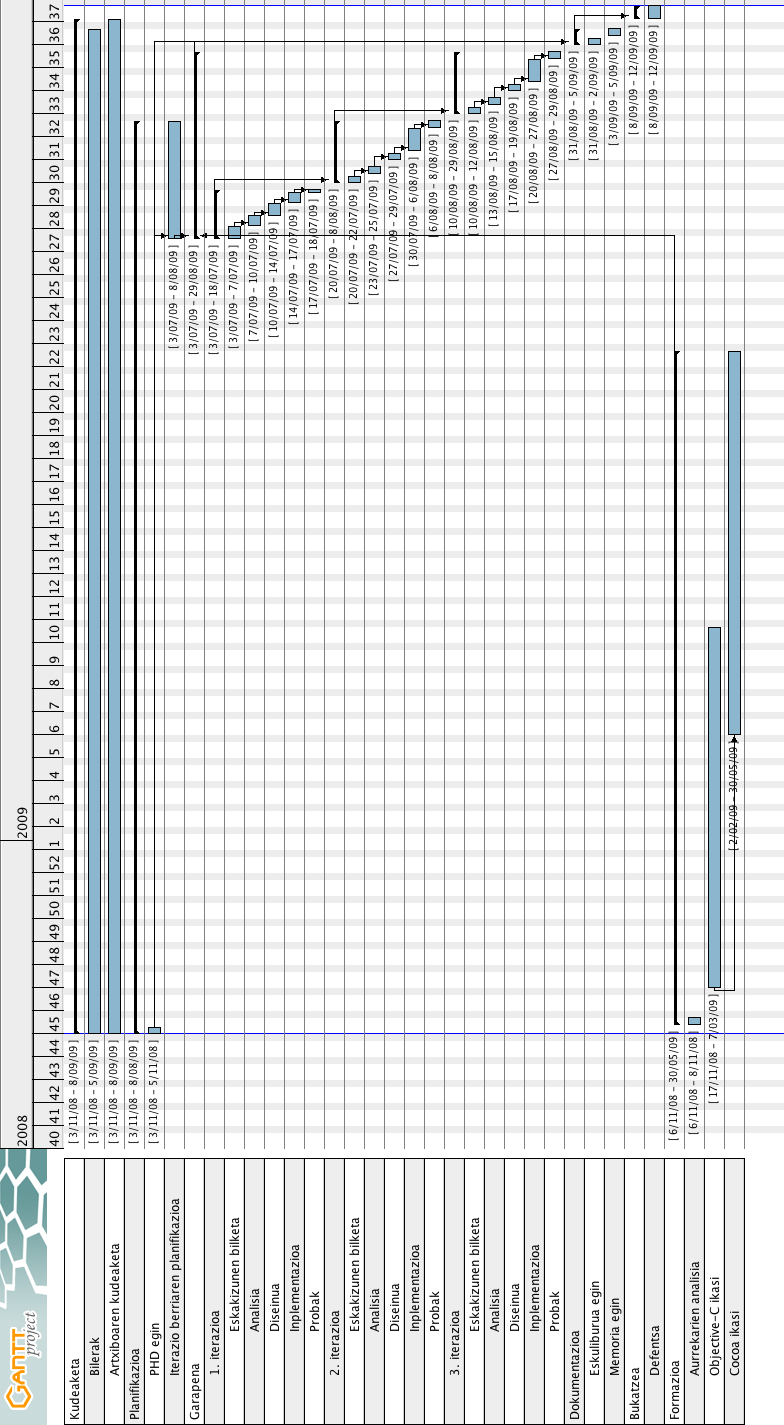
\includegraphics[width=\columnwidth, natwidth=784pt, natheight=1425pt]{Pictures/Chapter3/Gantt.png}
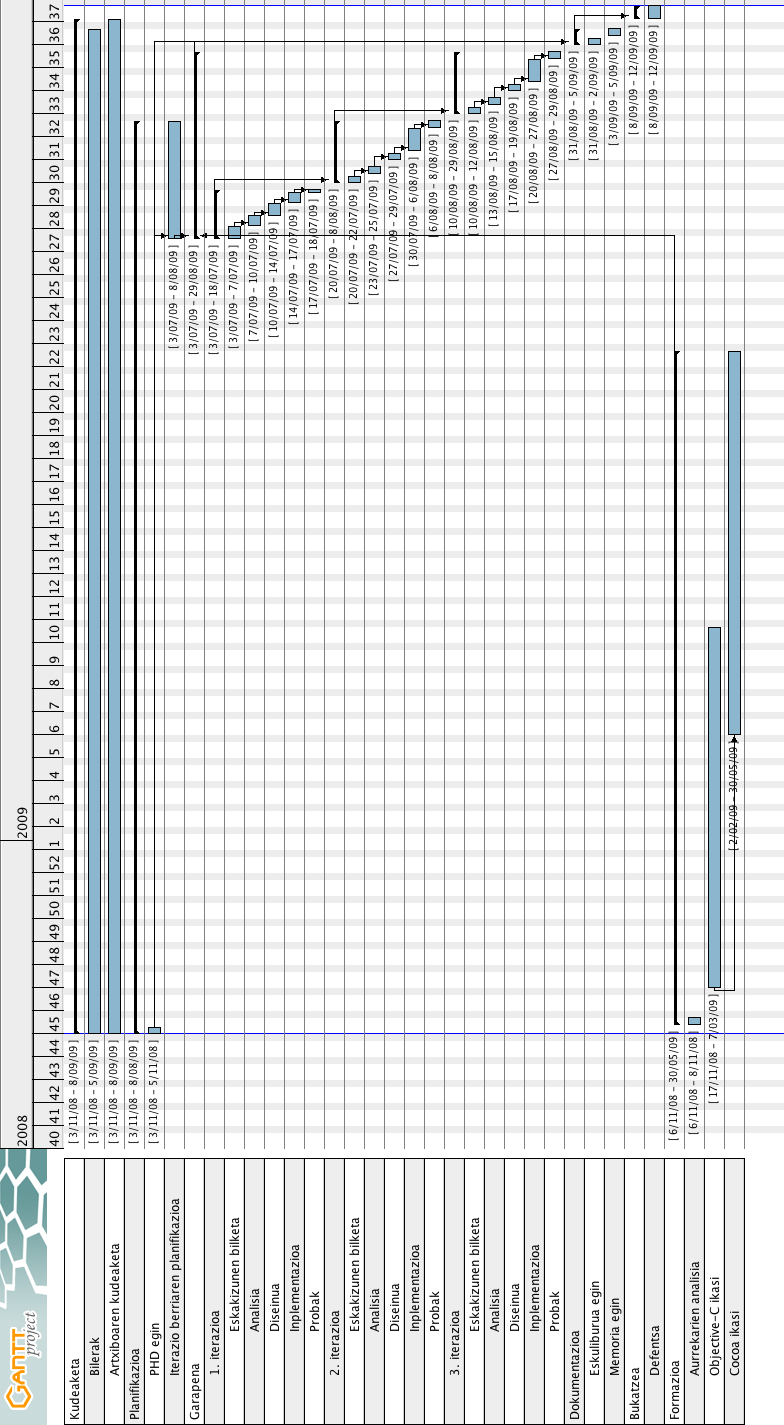
\includegraphics[scale=0.46]{Pictures/Chapter3/Gantt.png}
\caption{Gantt diagrama}
\label{gantt}
\end{center}
\end{figure}

\section{Arriskuak}
Proiektu guztietan kontuan hartu beharreko arriskuan agertzen dira, batzuk beste batzuk baino larriagoak eta gertatzeko probabilitate handiago edo txikiagokoak. Hauek dira aurreikusten diren arriskuak eta gertatzekotan zer egin behar den:
\begin{enumerate}
\item \textit{Atzerapenak proiektuan zehar:}\\
Proiektua garatzen den bitartean, ikaslea SIIT-eko 3. maila egiten egongo da, beraz bi ekintzak aldi berean egingo ditu. Honez gain, bere bizitza pertsonaleko beste aktibitate batzuk ere egingo ditu bitartean.\\
\textbf{Probabilitatea:} altua.\\
\textbf{Ondorioak:} planifikatutako emangarrien atzerapenak.\\
\textbf{Konponbidea:} datak birplanifikatu eta lan erritmoa igo ahal den einean.

\item \textit{Ikasle edo irakaslearen baja gaixotasunagatik:}\\
Ikaslea gaixotzen bada, ezin izango du proiektuan lan egin. Irakaslea aldiz gaixotzen bada, ezin izango du ikaslea gidatu proiektuan zehar.\\
\textbf{Probabilitatea:} baxua.\\
\textbf{Ondorioak:} planifikatutako emangarrien atzerapenak.\\
\textbf{Konponbidea:} esfortzua birplanifikatu entregatze datak betetzeko.

\item \textit{Lan egiteko zerbitzaria atzigarri ez egotea:}\\
Assembla.com erabiliko da garapenean zehar honen tresnak erabiliz, adibidez SVN zerbitzaria han egongo da. Software edo hardware arazoak direla eta agian ezin izango da atzitu denbora tarte batean.\\
\textbf{Probabilitatea:} baxua.\\
\textbf{Ondorioak:} egindako lanaren galera eta lana ezin egitea.\\
\textbf{Konponbidea:} aurretik sortutako babes kopiak erabiltzea.
\end{enumerate}

\section{Lan metodologia}
Proiektu honetan zehar jarraituko den metodologia softwarearen garapenerako prozesu bateratuak (\textbf{SGPB}) definitzen duena izango da. Modelatzeko lengoaia bezala \textit{Unified Modeling Language} (UML) erabiliko da.
\subsection{Bilerak}
Bilerak astean behin edo bi astero egingo dira, lan zamaren menpe. Bilera hauetan ikaslea eta proiektuaren zuzendaria egongo dira. Bertan egindako berrikusiko da planifikatutakoarekin bat datorren ikusteko eta hurrengo bileraren data esleituko da. Honez gain, denbora tarte horretan zein ataza egingo diren planifikatutko da.
\subsection{Teknologiak / Softwarea}
Proiektu honen garapenerako teknologia eta software hauek erabiliko ditugu:
\begin{itemize}
\item \textbf{\LaTeX{}:} dokumentazioa sortzeko markaketa lengoaia. WYSIWYM\footnote{\textit{What You See Is What You Mean} - Ikusten duzuna da egin nahi duzuna. \url{http://en.wikipedia.org/wiki/WYSIWYM}} motakoa da eta dokumentazioa teknikoa sortzeko oso erabilia da. Lana erraztearren, \textbf{itsas}\footnote{\url{http://itsas.ehu.es/}} taldeak eskaintzen duen txantiloia erabiliko da, bertan memoriak eduki behar duen formatua oso ondo definituta dagoelako eta lan asko aurreratuko digulako.

\LaTeX{} lengoaia da soilik, beraz editore bat eta konpiladore bat (iturburu fitxategietatik PDF fitxategi bat lortzeko) beharko ditugu. Editore bezala \textbf{MacVim}\footnote{\url{http://code.google.com/p/macvim}} erabiliko da, Mac OS X-erako vim editore famatuaren bertsio bat. Konpilatzeko \textbf{Mac\TeX}\footnote{\url{http://www.tug.org/mactex/}} distribuzioa erabiliko da, bertan beharko ditugun tresna eta plugin guztiak aurkituko ditugulako.
\item \textbf{iWork:} ofimatikarako suite bat. Nahiz eta \LaTeX{} erabili dokumentazioa sortzeko, behar bada erabili behar izango dugu, adibidez grafikoak sortzeko.
\item \textbf{Dia:} diagramak sortzeko tresna. Gure kasuan UML erabiliko dugunez zenbait diagrama sortu beharko ditugu proiektuan zehar: LDE, EKE, sekuentzia diagramak, klase diagramak, etab.
\item \textbf{GanttProject:} Gantt diagrama sortzeko erabiliko dugu, hau da, proiektuaren ataza desberdinen iraupena deskribatzeko.
\item \textbf{Objective-C 2.0:} objektuei zuzendutako programazio lengoaia, C lengoaiaren gainean eratua. Mac OS X sisteman aplikazioak garatzeko programazio lengoaia erabiliena da. Konpilatzeko ez dugu ezer berezirik behar, \textbf{gcc} konpiladore famatua erabili daitekeelako.

2.0 bertsioan asko lagunduko diguten funtzionalitateak aurkituko ditugu: zabor bilketa, propietateak, \textit{fast enumeration}, etab.
\item \textbf{Cocoa:} objektuei zuzendutako API\footnote{Application Programming Interface} natiboa Mac OS X sistemarako. Objective-C lengoaia erabiltzen du eta sistemarekin bikain integratzen dira API hau erabiltzen duten aplikazioak.
\item \textbf{Xcode:} aplikazioa garatzeko IDE\footnote{Integrated Development Environment}-a. Beste IDE gehienetan aurkitu ditzakegun funtzionalitateak dauzka (araztailea, sintaxi koloreztailea, etab.).
\item \textbf{Interface Builder:} Cocoa aplikazioen interfaze grafikoak eratzeko eta kodearekin \textit{lotzeko} aplikazioa. Bi aplikazio hauek eta gcc konpiladorea Apple-ek eskaintzen ditu dohain: \url{http://developer.apple.com/Tools/}.
\end{itemize} 
\section{Bideragarritasuna}
Ekonomikoki proiektua bideragarria da, ez dugulako dirurik inbertitu behar, garapenerako ekipoak baditugulako. Sistema eragilea kenduta, erabiliko diren tresna eta teknologia guztiak dohainekoak dira, eta horietako batzuk gainera askeak dira.

% TODO: feo feo
Ikuspegi teknologikoa kontuan hartuta ere bideragarria da, egin nahi duguna inplementatuta dagoelako beste sistema eragile batzuetan.

Azkenik, denboraren ikus puntutik, kurtsoan zehar egitea ezinezkoa izango da, ikasleak duen lan zamagatik, beraz, proiektuaren zati handiena udan egin behar izango da, ekaineko azterketak bukatu ondoren. Plangintzaren arabera iraileko bigarren asterako prest egon beharko da. % 3. Kapitulua: Proiektuaren helburu dokumentua
\tocchapter{Softwarearen garapenerako prozesu bateratua}

\section{Eskakizunen bilketa}
Gure aplikazioak eduki behar dituen eskakizun funtzionalak zehazteko, hau da, aktoreen beharrak zerrendatzeko, balio du eskakizunen bilketak. Gure kasuan aktore bakarra izango dugu, \textbf{erabiltzailea} hain zuzen ere. Hauek dira bere eskakizunak:
\subsection{Azpitituluen inguruko eskakizunak}
\begin{itemize}
\item ASS eta SRT motako azpitituluak irekitzea eta gordetzea.
\item Azpititulu fitxategi berriak sortzeko aukera.
\item TXT fitxategietatik dialogoak inportatzea.
\item Fitxategiaren goiburukoen edizioa.
\item Lerro bakoitzaren eremuen gaineko edizioa: aktorea, estiloa, testua, denborak, etab. aldatzea.
\item Lerroen gaineko eragiketak: gehitu, kendu, \textit{shift}, \textit{split}, \textit{join}, bikoiztu, etab.
\item Sintaxia nabarmendua erosoago lan egiteko: ASS komandoen identifikazioa eta koloreztatzea.
\end{itemize}
\subsection{\textit{Typesetting}-aren inguruko eskakizunak}
\begin{itemize}
\item Estilo editorea estilo berriak sortzeko edo daudenak aldatzeko.
\item Estilo kudeatzailea, estiloak gorde ahal izateko edo \textit{script} batean txertatzeko.
\end{itemize}
\subsection{Tresna edo laguntzaileen inguruko eskakizunak}
\begin{itemize}
\item Itzulpenak egiteko laguntzailea.
\item Zuzentzaile ortografikoa.
\item Estiloak aplikatzeko laguntzailea.
\end{itemize}
\subsection{Bestelako eskakizunak}
\begin{itemize}
\item Lana periodikoki gordetzea modu automatikoan.
\item Dokumentu anitz irekita edukitzea aldi berean.
\item Undo/Redo aukerak.
\end{itemize}

\section{Analisia}
Nahiz eta programak zenbait formaturekin lan egin ahalko duen (ASS, SRT eta TXT), formatu \textit{natiboa} ASS izango da. Honen arrazoia zera da: ASS formatuak badauka SRT eta TXT formatuek eskaintzen duten guztia, baina alderantziz ez, hau da, ASS formatua askoz aurreratuagoa da. 

\begin{figure}[htp]
\begin{center}
%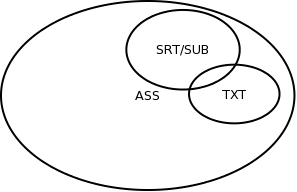
\includegraphics[width=\columnwidth, natwidth=555pt, natheight=402pt]{Pictures/Chapter4/Analisia/formatuak.png}
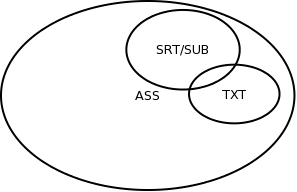
\includegraphics[scale=0.5]{Pictures/Chapter4/Analisia/formatuak.png}
\caption{Azpititulu formatuak}
\label{formatuak}
\end{center}
\end{figure}

\ref{formatuak}~Irudian ikusten denez, SRT eta TXT formatuak ASS formatuaren azpimultzoak direla esan daiteke. SRT formatuak dialogoak eta hauen hasiera eta bukaera denborak dauzka, eta TXT formatuak ordea, dialogoak eta hauen aktoreak bakarrik eskaintzen ditu.
\subsection{Domeinuaren eredua}
\ref{de}~Irudian ikusten denez, domeinuko osagaien izenak ingeleraz daude, honako arrazoiengatik: alde batetik, ASS formatuaren espezifikazioan izenak ingeleraz agertzen direlako\cite{gu:ass}, eta bestetik programa askea izango denez, norbaitek kodea irakurri edo hobetu nahi badu, ia ziurrena ingelera jakingo du euskara baino.
\begin{figure}[htp]
\begin{center}
%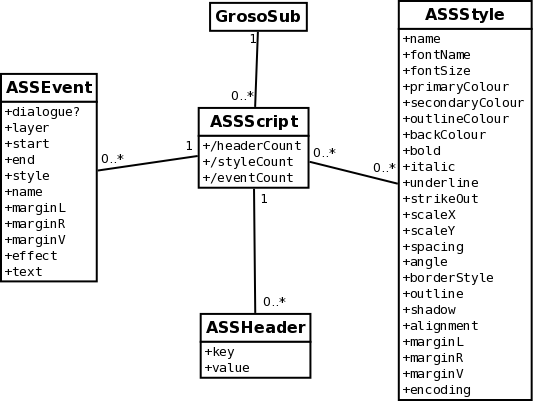
\includegraphics[width=\columnwidth, natwidth=555pt, natheight=402pt]{Pictures/Chapter4/Analisia/DE.png}
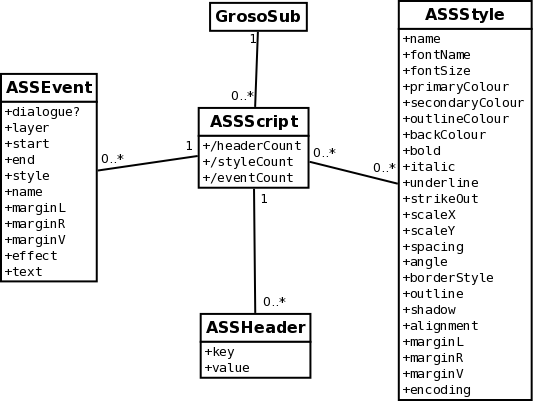
\includegraphics[scale=0.35]{Pictures/Chapter4/Analisia/DE.png}
\caption{Domeinuaren eredua}
\label{de}
\end{center}
\end{figure}

ASSScript da gure entitate nagusia eta ASS formatuko fitxategi bat errepresentatuko du. Fitxategiaren barruan goiburukoak, estiloak eta gertakizunak aurkituko ditugu, beraz hauetako bakoitza entitate desberdinetan banatuta daude (ASSEvent, ASSHeader eta ASSStyle). ASSEvent eta ASSHeader bakoitza ASSScript batekoa izango da, eta ASSScript-ak hauetako 0 edo gehiago edukiko ditu barnean. ASSScript batek 0 estilo edo gehiago edukiko ditu, eta hauek 0 ASSScript edo gehiagokoen parte izango dira, beste biekin alderatuta estilo biltegiak edukiko ditugulako. Azkenik, gure aplikazioak 0 ASSScript edo gehiago maneiatu ahal izango ditu aldi berean.

\subsection{Egoera diagrama}
Programaren izaera dela eta, egoera desberdinekin aurkituko gara. Definituko diren egoeratan zenbait erabilpen kasu gauzatu ahalko ditugu, batzuetan egoeraz aldatuz. Honako diagraman ikus daitezke egoerak:

\begin{figure}[htp]
\begin{center}
%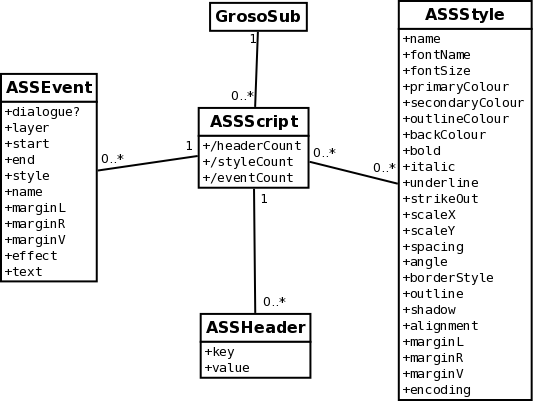
\includegraphics[width=\columnwidth, natwidth=555pt, natheight=402pt]{Pictures/Chapter4/Analisia/DE.png}
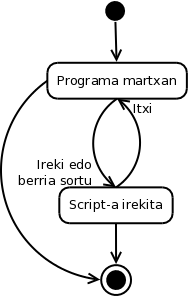
\includegraphics[scale=0.4]{Pictures/Chapter4/Analisia/ED.png}
\caption{Egoera diagrama}
\label{ed}
\end{center}
\end{figure}
\newpage
\subsection{Erabilpen kasuak}
\subsubsection{Egoera guztietan egin daitezkeenak}
\begin{figure}[htp]
\begin{center}
%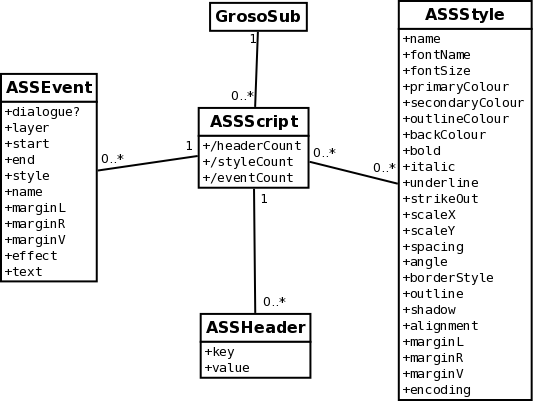
\includegraphics[width=\columnwidth, natwidth=555pt, natheight=402pt]{Pictures/Chapter4/Analisia/DE.png}
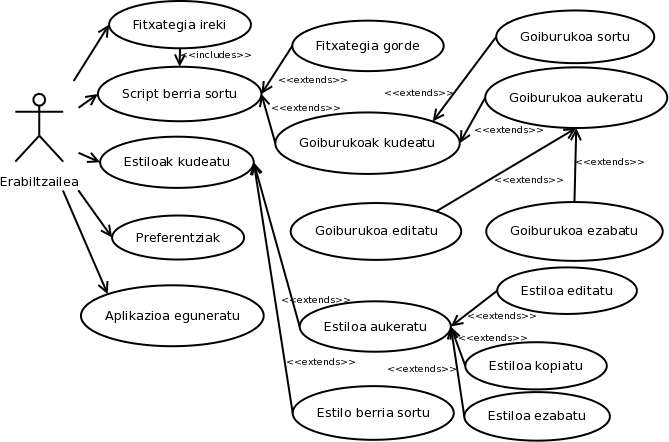
\includegraphics[scale=0.4]{Pictures/Chapter4/Analisia/EKE-Guztiak.png}
\caption{EKE - Egoera guztiak}
\label{eke-guztiak}
\end{center}
\end{figure}
\noindent\\
\textbf{ID:} G01.\\
\textbf{Erabilpen kasua:} Fitxategia ireki.\\
\textbf{Aktoreak:} Erabiltzailea.\\
\textbf{Deskribapena:} Fitxategi sisteman dagoen fitxategi bat kargatzen du.\\
\textbf{Aurrebaldintzak:} Fitxategia existitzen da.\\
\textbf{Postbaldintzak:} Fitxategia kargatuta geratzen da.\\
\textbf{Gertaera fluxu normala:}
\begin{enumerate}
	\item \textit{Erabiltzailea:} Fitxategi sistemako fitxategi bat aukeratzen du.
	\item \textit{Sistema:} Script berri bat sortzen du (\underline{includes: G02}).
	\item \textit{Sistema:} Sortu berri duen script-ean aukeratutako fitxategiko datuak kargatzen ditu.
	\item \textit{Sistema:} Erabiltzaileari erakusten dio lehio berri batean.
\end{enumerate}
\textbf{Gertaera fluxu alternatiboa:}
\begin{itemize}
	\item 3. urratsa: fitxategiaren formatua ez da zuzena.
		\begin{enumerate}
		\item \textit{Sistema:} Erabiltzaileari errorearen berri emango dio.
		\item \textit{Erabiltzailea:} Fitxategi berri bat aukeratuko du edo erabilpen kasutik aterako da.
		\end{enumerate}
\end{itemize}
\line(1,0){390}\\
\noindent\\
\textbf{ID:} G02.\\
\textbf{Erabilpen kasua:} Script berria sortu.\\
\textbf{Aktoreak:} Erabiltzailea.\\
\textbf{Deskribapena:} Script berri bat sortzen da defektuzko balioekin.\\
\textbf{Aurrebaldintzak:}\\
\textbf{Postbaldintzak:} Script-a sortzen da eta erabiltzaileari erakusten zaio.\\
\textbf{Gertaera fluxu normala:}
\begin{enumerate}
	\item \textit{Sistema:} Script berria sortzen du eta defektuzko informazioarekin osatzen du.
	\item \textit{Sistema:} Erabiltzaileari erakusten dio lehio berri batean.
\end{enumerate}
%\line(1,0){390}\\
\noindent\\
\textbf{ID:} G03.\\
\textbf{Erabilpen kasua:} Fitxategia gorde.\\
\textbf{Aktoreak:} Erabiltzailea.\\
\textbf{Deskribapena:} Irekita dagoen script-a fitxategi batean gordetzen du aukeratutako formatuan.\\
\textbf{Aurrebaldintzak:} Script-a irekita dago.\\
\textbf{Postbaldintzak:} Script-a fitxategi sistemako fitxategi batean gordeta geratzen da.\\
\textbf{Gertaera fluxu normala:}
\begin{enumerate}
	\item \textit{Erabiltzailea:} Gordetzeko izena, lekua eta formatua aukeratuko ditu.
	\item \textit{Sistema:} Dagokion formatuan gordeko du irekita dagoen script-a.
\end{enumerate}
\line(1,0){390}\\
\noindent\\
\textbf{ID:} G04.\\
\textbf{Erabilpen kasua:} Goiburukoak kudeatu.\\
\textbf{Aktoreak:} Erabiltzailea.\\
\textbf{Deskribapena:} Irekita dagoen script-aren goiburukoak editatzen ditu.\\
\textbf{Aurrebaldintzak:} Script-a irekita dago.\\
\textbf{Postbaldintzak:} Goiburukoetan egindako aldaketak script-ean gordeta geratuko dira.\\
\textbf{Gertaera fluxu normala:}
\begin{enumerate}
	\item \textit{Sistema:} Script-ean dauden goiburuak zerrendatuko ditu.
	\item \textit{Erabiltzailea:} Goiburuko bat aukeratuko du editatzeko edo ezabatzeko, edo goiburuko berri bat sortuko du.
	\item \textit{Sistema:} Erabiltzaileak aukeratutako ekintza egingo du.
	\item \textit{Erabiltzailea:} Berriro egiteko edo irtetzeko aukera izango du.
	\item \textit{Sistema:} egin diren aldaketak script-ean gordeko ditu.
\end{enumerate}
\textbf{Gertaera fluxu alternatiboa:}
\begin{itemize}
	\item 4. urratsa: berriro egitea aukeratuko du erabiltzaileak:
		\begin{enumerate}
		\item \textit{Sistema:} Goiburukoen zerrenda eguneratuko du egin den azken aldaketa bertan isladatzeko.
		\item \textit{Erabiltzailea:} Beste goiburuko bat aukeratuko du editatzeko edo ezabatzeko, edo goiburuko berri bat sortuko du.
		\end{enumerate}
\end{itemize}
\line(1,0){390}\\
\noindent\\
\textbf{ID:} G05.\\
\textbf{Erabilpen kasua:} Goiburukoa sortu.\\
\textbf{Aktoreak:} Erabiltzailea.\\
\textbf{Deskribapena:} Irekita dagoen script-ean goiburuko berri bat sortzen du.\\
\textbf{Aurrebaldintzak:} Goiburukoen kudeatzailea martxan dago.\\
\textbf{Postbaldintzak:} Goiburuko berria goiburukoen zerrendan gordeko da.\\
\textbf{Gertaera fluxu normala:}
\begin{enumerate}
	\item \textit{Sistema:} Goiburuko berria sortzen du defektuzko balioekin eta goiburukoen zerrendan gordeko du.
\end{enumerate}
\line(1,0){390}\\
\noindent\\
\textbf{ID:} G06.\\
\textbf{Erabilpen kasua:} Goiburukoa aukeratu.\\
\textbf{Aktoreak:} Erabiltzailea.\\
\textbf{Deskribapena:} Goiburuko bat aukeratzen du honekin zenbait eragiketa egin ahal izateko.\\
\textbf{Aurrebaldintzak:} Goiburukoen kudeatzailea martxan dago.\\
\textbf{Postbaldintzak:} Goiburuko bat aukeratuta geratzen da.\\
\textbf{Gertaera fluxu normala:}
\begin{enumerate}
	\item \textit{Erabiltzailea:} Goiburuko bat aukeratuko du goiburukoen zerrendatik.
	\item \textit{Sistema:} Erabiltzaileak aukeratutako goiburukoa markatuko du interfazean.
\end{enumerate}
\line(1,0){390}\\
\noindent\\
\textbf{ID:} G07.\\
\textbf{Erabilpen kasua:} Goiburukoa editatu.\\
\textbf{Aktoreak:} Erabiltzailea.\\
\textbf{Deskribapena:} Aukeratutako goiburukoaren balioa aldatzen du.\\
\textbf{Aurrebaldintzak:} Goiburuko bat aukeratuta dago.\\
\textbf{Postbaldintzak:} Aukeratutako goiburukoa aldatuta geratzen da script-ean.\\
\textbf{Gertaera fluxu normala:}
\begin{enumerate}
	\item \textit{Sistema:} Aukeratutako goiburukoaren balioa erakusten du.
	\item \textit{Erabiltzailea:} Balio berria sartzen du.
	\item \textit{Sistema:} Erabiltzaileak sartutako balioa goiburukoen zerrendan gordetzen du.
\end{enumerate}
\line(1,0){390}\\
\noindent\\
\textbf{ID:} G08.\\
\textbf{Erabilpen kasua:} Goiburukoa ezabatu.\\
\textbf{Aktoreak:} Erabiltzailea.\\
\textbf{Deskribapena:} Aukeratutako goiburukoa ezabatzen du script-etik.\\
\textbf{Aurrebaldintzak:} Goiburuko bat aukeratuta dago.\\
\textbf{Postbaldintzak:} Goiburukoa ezabatuko da script-etik.\\
\textbf{Gertaera fluxu normala:}
\begin{enumerate}
	\item \textit{Sistema:} Goiburukoa zerrendatik ezabatuko du.
\end{enumerate}
\line(1,0){390}\\
\noindent\\
\textbf{ID:} G09.\\
\textbf{Erabilpen kasua:} Estiloak kudeatu.\\
\textbf{Aktoreak:} Erabiltzailea.\\
\textbf{Deskribapena:} Estilo kudeatzailea agertuko da, script-ean eta biltegian dauden estiloak kudeatzeko.\\
\textbf{Aurrebaldintzak:} Script-a kargatuta dago.\\
\textbf{Postbaldintzak:} Estilo kudeatzailea kargatuko da.\\
\textbf{Gertaera fluxu normala:}
\begin{enumerate}
	\item \textit{Sistema:} Biltegian dauden estiloak eta script-ean daudenak zerrendatuko ditu.
	\item \textit{Sistema:} Estiloak kudeatzeko kontrolak kargatuko ditu.
\end{enumerate}
\line(1,0){390}\\
\noindent\\
\textbf{ID:} G10.\\
\textbf{Erabilpen kasua:} Estilo berria sortu.\\
\textbf{Aktoreak:} Erabiltzailea.\\
\textbf{Deskribapena:} Estilo berria sortuko eta editatuko du.\\
\textbf{Aurrebaldintzak:} Estilo kudeatzailean dago programa.\\
\textbf{Postbaldintzak:} Estiloa gordeta geratuko da.\\
\textbf{Gertaera fluxu normala:}
\begin{enumerate}
	\item \textit{Erabiltzailea:} Estiloa script-ean edo biltegian gordetzea aukeratuko du.
	\item \textit{Sistema:} Estilo berri bat sortuko du defektuzko aukerekin.
	\item \textit{Sistema:} Sortu berri duen estiloa editatzeko aukera emango dio erabiltzaileari (\underline{includes G12}).
	\item \textit{Sistema:} Estiloa gordeko du aukeratutako tokian.
\end{enumerate}
\line(1,0){390}\\
\noindent\\
\textbf{ID:} G11.\\
\textbf{Erabilpen kasua:} Estiloa aukeratu.\\
\textbf{Aktoreak:} Erabiltzailea.\\
\textbf{Deskribapena:} Biltegian edo script-ean dagoen estilo bat aukeratzen du ondoren eragiketaren bat egiteko.\\
\textbf{Aurrebaldintzak:} Estilo kudeatzailean dago programa.\\
\textbf{Postbaldintzak:} Estiloa aukeratuta geratzen da.\\
\textbf{Gertaera fluxu normala:}
\begin{enumerate}
	\item \textit{Erabiltzailea:} Biltegiko edo script-eko estilo zerrendan dagoen estilo bat aukeratzen du.
	\item \textit{Sistema:} Erabiltzaileak aukeratutako estiloa markatzen du interfazean eta dagozkion kontrolak aktibatzen ditu.
\end{enumerate}
\line(1,0){390}\\
\noindent\\
\textbf{ID:} G12.\\
\textbf{Erabilpen kasua:} Estiloa editatu.\\
\textbf{Aktoreak:} Erabiltzailea.\\
\textbf{Deskribapena:} Aukeratutako estiloaren eremuak editatzen ditu.\\
\textbf{Aurrebaldintzak:} Estilo bat aukeratuta dago.\\
\textbf{Postbaldintzak:} Estiloa gordetzen du dagokion lekuan aldaketa berriekin.\\
\textbf{Gertaera fluxu normala:}
\begin{enumerate}
	\item \textit{Sistema:} Aukeratutako estiloaren eremuak eta hauen balioak pantailaratzen ditu.
	\item \textit{Erabiltzailea:} Eremu bat aukeratzen du eta bere balioa aldatzen du.
	\item \textit{Erabiltzailea:} Beste eremu bat aukeratu (2. urratsa) edo irten daiteke.
	\item \textit{Sistema:} Estiloa gordetzen du.
\end{enumerate}
\line(1,0){390}\\
\noindent\\
\textbf{ID:} G13.\\
\textbf{Erabilpen kasua:} Estiloa kopiatu.\\
\textbf{Aktoreak:} Erabiltzailea.\\
\textbf{Deskribapena:} Estiloa kopiatzen du biltegitik script-era edo alderantziz.\\
\textbf{Aurrebaldintzak:} Estilo bat aukeratuta dago.\\
\textbf{Postbaldintzak:} Estiloa kopiatzen da.\\
\textbf{Gertaera fluxu normala:}
\begin{enumerate}
	\item \textit{Sistema:} Estiloa kopiatzen du leku batetik bestera.
	\item \textit{Sistema:} Estilo zerrenda eguneratzen du.
\end{enumerate}
\textbf{Gertaera fluxu alternatiboa:}
\begin{itemize}
	\item 1. urratsa: helburuan badago izen berdineko estiloa:
		\begin{enumerate}
		\item \textit{Sistema:} Izen berria emango dio estiloari, zenbaki bat parentesi tartean txertatuz izenaren amaieran.
		\end{enumerate}
\end{itemize}
\line(1,0){390}\\
\noindent\\
\textbf{ID:} G14.\\
\textbf{Erabilpen kasua:} Estiloa ezabatu.\\
\textbf{Aktoreak:} Erabiltzailea.\\
\textbf{Deskribapena:} Aukeratutako estiloa dagokion tokitik ezabatzen du.\\
\textbf{Aurrebaldintzak:} Estilo bat aukeratuta dago.\\
\textbf{Postbaldintzak:} Estiloa ezabatzen da.\\
\textbf{Gertaera fluxu normala:}
\begin{enumerate}
	\item \textit{Sistema:} Estiloa ezabatuko du dagokion lekutik.
\end{enumerate}
\line(1,0){390}\\
\noindent\\
\textbf{ID:} G15.\\
\textbf{Erabilpen kasua:} Preferentziak.\\
\textbf{Aktoreak:} Erabiltzailea.\\
\textbf{Deskribapena:} Programaren preferentziak aldatzen ditu.\\
\textbf{Aurrebaldintzak:}\\
\textbf{Postbaldintzak:} Programaren preferentziak aldatuta gordetzen ditu.\\
\textbf{Gertaera fluxu normala:}
\begin{enumerate}
	\item \textit{Sistema:} Preferentziak erakutsiko ditu momentu horretan dituen balioekin.
	\item \textit{Erabiltzailea:} Nahi dituen balioak aldatuko ditu eta preferentzia lehioa itxiko du.
	\item \textit{Sistema:} Erabiltzaileak jarri dituen balioak gorde eta aplikatuko ditu.
\end{enumerate}
\line(1,0){390}\\
%\newpage
\noindent\\
\textbf{ID:} G16.\\
\textbf{Erabilpen kasua:} Aplikazioa eguneratu.\\
\textbf{Aktoreak:} Erabiltzailea.\\
\textbf{Deskribapena:} Aplikazioaren bertsio berriagoak bilatuko ditu eta eguneratzeko aukera emango du.\\
\textbf{Aurrebaldintzak:} Internet-eko konexioa egon behar da.\\
\textbf{Postbaldintzak:} Aplikazioa eguneratzen du erabiltzaileak horrela nahi badu.\\
\textbf{Gertaera fluxu normala:}
\begin{enumerate}
	\item \textit{Sistema:} Aplikazioaren eguneraketak daude begiratuko du. Baldin badaude eguneraketaren informazioa erakutsiko du.
	\item \textit{Erabiltzailea:} Aplikazioa eguneratu nahi duela baieztatuko du.
	\item \textit{Sistema:} Eguneraketa jaitsi eta instalatuko du.
	\item \textit{Sistema:} Aplikazioa berrabiaraziko du eguneraketa berriekin.
\end{enumerate}
\newpage
\subsubsection{\textit{Script-a irekita} egoerakoak}
\begin{figure}[htp]
\begin{center}
%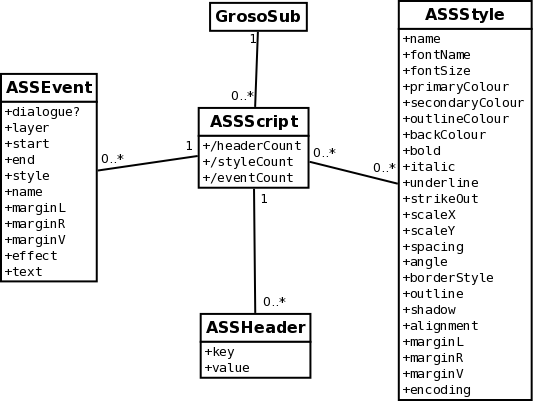
\includegraphics[width=\columnwidth, natwidth=555pt, natheight=402pt]{Pictures/Chapter4/Analisia/DE.png}
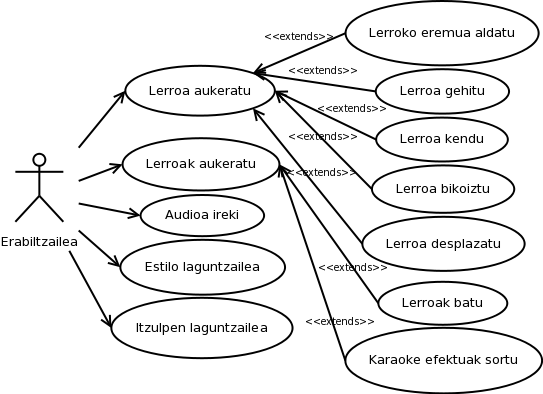
\includegraphics[scale=0.4]{Pictures/Chapter4/Analisia/EKE-Script.png}
\caption{EKE - Script-a irekita egoera}
\label{eke-script}
\end{center}
\end{figure}
\noindent\\
\textbf{ID:} S01.\\
\textbf{Erabilpen kasua:} Lerroak aukeratu.\\
\textbf{Aktoreak:} Erabiltzailea.\\
\textbf{Deskribapena:} Script-ean dagoen lerro bat edo gehiago aukeratzen ditu ondoren bere gainean zenbait eragiketa egiteko.\\
\textbf{Aurrebaldintzak:}  Script-a kargatuta dago eta gutxienez lerro bat dauka.\\
\textbf{Postbaldintzak:} Lerroak aukeratuta geratzen dira.\\
\textbf{Gertaera fluxu normala:}
\begin{enumerate}
	\item \textit{Erabiltzailea:} Script-ean dagoen lerro bat edo gehiago aukeratuko ditu.
	\item \textit{Sistema:} Erabiltzaileak aukeratutako lerroak markatuko ditu interfazean.
	\item \textit{Sistema:} Lerro bakarra aukeratu bada, honen datuak kargatuko ditu interfazean.
\end{enumerate}
\line(1,0){390}\\
\noindent\\
\textbf{ID:} S02.\\
\textbf{Erabilpen kasua:} Lerroko eremua aldatu.\\
\textbf{Aktoreak:} Erabiltzailea.\\
\textbf{Deskribapena:} Aukeratutako lerroko eremu baten edukia aldatzen du.\\
\textbf{Aurrebaldintzak:} Lerro bat aukeratuta dago.\\
\textbf{Postbaldintzak:} Aldatutako eremua lerroan gordeta geratuko da.\\
\textbf{Gertaera fluxu normala:}
\begin{enumerate}
	\item \textit{Sistema:} Aukeratutak lerroaren eremu guztiak eta hauen balioak erakutsiko ditu.
	\item \textit{Erabiltzailea:} Eremu bat aukeratuko du eta honen balioa aldatuko du.
	\item \textit{Erabiltzailea:} Beste eremu bat aldatzeko (2. urratsera) edo aldaketak gordetzeko agindua emango du.
	\item \textit{Sistema:} Lerroan egindako aldaketak gordeko dira.
\end{enumerate}
\line(1,0){390}\\
\noindent\\
\textbf{ID:} S03.\\
\textbf{Erabilpen kasua:} Lerroa gehitu.\\
\textbf{Aktoreak:} Erabiltzailea.\\
\textbf{Deskribapena:} Lerro berri bat gehituko du script-ean.\\
\textbf{Aurrebaldintzak:} Lerro bat aukeratuta dago.\\
\textbf{Postbaldintzak:} Lerro berria script-ean gehituko da.\\
\textbf{Gertaera fluxu normala:}
\begin{enumerate}
	\item \textit{Erabiltzailea:} Aukeratutako lerroaren aurrean edo atzean sartzeko aukeratuko du.
	\item \textit{Sistema:} Erabiltzaileak aukeratutako lekuan txertatuko du lerro berria defektuzko informazioarekin.
\end{enumerate}
\textbf{Gertaera fluxu alternatiboa:}
\begin{itemize}
	\item 0. urratsa: ez badago lerrorik aukeratuta script-ean:
		\begin{enumerate}
		\item \textit{Sistema:} Lerro berri bat gehituko du.
		\end{enumerate}
\end{itemize}
\line(1,0){390}\\
\noindent\\
\textbf{ID:} S04.\\
\textbf{Erabilpen kasua:} Lerroa kendu.\\
\textbf{Aktoreak:} Erabiltzailea.\\
\textbf{Deskribapena:} Aukeratutako lerroa script-etik ezabatzen du.\\
\textbf{Aurrebaldintzak:} Lerro bat aukeratuta dago.\\
\textbf{Postbaldintzak:} Lerroa script-etik ezabatuko da.\\
\textbf{Gertaera fluxu normala:}
\begin{enumerate}
	\item \textit{Sistema:} Erabiltzaileak aukeratutako lerroa ezabatuko du script-etik
\end{enumerate}
\line(1,0){390}\\
\noindent\\
\textbf{ID:} S05.\\
\textbf{Erabilpen kasua:} Lerroa bikoiztu.\\
\textbf{Aktoreak:} Erabitzailea.\\
\textbf{Deskribapena:} Aukeratutako lerroaren kopia bat egingo du aukeratutako lerroaren azpian.\\
\textbf{Aurrebaldintzak:} Lerro bat aukeratuta dago.\\
\textbf{Postbaldintzak:} Aukeratutako lerroa bikoiztuta geratuko da.\\
\textbf{Gertaera fluxu normala:}
\begin{enumerate}
	\item \textit{Sistema:} Lerro berri bat sortuko du aukeratutakoaren azpian eta bertan aukeratutako lerroaren datuak sartuko ditu.
\end{enumerate}
\line(1,0){390}\\
\noindent\\
\textbf{ID:} S06.\\
\textbf{Erabilpen kasua:} Lerroak desplazatu.\\
\textbf{Aktoreak:} Erabiltzailea.\\
\textbf{Deskribapena:} Aukeratutako lerroen denborak desplazatzen ditu.\\
\textbf{Aurrebaldintzak:} Gutxienez lerro bat aukeratuta dago.\\
\textbf{Postbaldintzak:} Aukeratutako lerroen denborak desplazatuta geratzen dira.\\
\textbf{Gertaera fluxu normala:}
\begin{enumerate}
	\item \textit{Sistema:} Lerroak desplazatzeko aukerak erakutsiko ditu interfazean.
	\item \textit{Erabiltzailea:} Desplazatu nahi dituen denborak (hasiera denbora, bukaera denbora edo biak) eta zenbat desplazatu nahi dituen aukeratuko du.
	\item \textit{Sistema:} Aukeratutako lerroen denborak aldatuko ditu erabiltzaileak emandako datuekin.
\end{enumerate}
%\line(1,0){390}\\
\noindent\\
\textbf{ID:} S07.\\
\textbf{Erabilpen kasua:} Lerroak batu.\\
\textbf{Aktoreak:} Erabiltzailea.\\
\textbf{Deskribapena:} Aukeratuta dauden lerroak kateatzen ditu.\\
\textbf{Aurrebaldintzak:} 2 lerro gutxienez aukeratuta daude.\\
\textbf{Postbaldintzak:} Aukeratako lerroak kateatuta dituen lerro berri bat sortzen da.\\
\textbf{Gertaera fluxu normala:}
\begin{enumerate}
	\item \textit{Sistema:} Lerro berri bat sortzen du.
	\item \textit{Sistema:} Aukeratutako lerroen edukia (testua) kateatzen du eta denborak egokitzen ditu (hasiera denboren minimoa eta bukaera denboren maximoa).
	\item \textit{Sistema:} Aukeratutako lerroak ezabatzen ditu.
\end{enumerate}
\line(1,0){390}\\
\noindent\\
\textbf{ID:} S08.\\
\textbf{Erabilpen kasua:} Estilo laguntzailea.\\
\textbf{Aktoreak:} Erabiltzailea.\\
\textbf{Deskribapena:} Estilo laguntzailea kargatuko du estiloak aplikatzeko.\\
\textbf{Aurrebaldintzak:} Script-a kargatuta dago.\\
\textbf{Postbaldintzak:} Estiloak esleituko zaizkie aukeratutako lerroei.\\
\textbf{Gertaera fluxu normala:}
\begin{enumerate}
	\item \textit{Sistema:} Script-ean dauden estiloak eta uneko lerroaren testua eta aktorea erakutsiko ditu interfazean.
	\item \textit{Erabiltzailea:} Sagua edo teklatuaren bidez estilo bat aukeratuko du.
	\item \textit{Sistema:} Uneko lerroari aukeratutako estiloa ezarriko dio eta hurrengo lerroa kargatuko du interfazean.
\end{enumerate}
\line(1,0){390}\\
\noindent\\
\textbf{ID:} S09.\\
\textbf{Erabilpen kasua:} Itzulpen laguntzailea.\\
\textbf{Aktoreak:} Erabiltzailea.\\
\textbf{Deskribapena:} Itzulpen laguntzailea kargatuko du.\\
\textbf{Aurrebaldintzak:} Script-a kargatuta dago.\\
\textbf{Postbaldintzak:} Erabiltzaileak egindako itzulpenak ezarriko dira.\\
\textbf{Gertaera fluxu normala:}
\begin{enumerate}
	\item \textit{Sistema:} Uneko lerroaren testua erakutsiko du interfazean.
	\item \textit{Erabiltzailea:} Lerro horren itzulpena sartuko du.
	\item \textit{Sistema:} Uneko lerroaren testua aldatuko du erabiltzaileak sartu duenarekin eta hurrengo lerroa erakutsiko du interfazean.
\end{enumerate}

\newpage
\section{Diseinua}
\subsection{Dokumentuetan oinarritutako aplikazioak}
Gure aplikazioak oso komunak diren funtzionalitate batzuk izan behar ditu: fitxategiak ireki, berriak sortu, itxi, etab. Aplikazio hauek dokumentuetan oinarritutakoak dira, eta oso komunak direnez, Cocoa API-ak hauek garatzeko erreztasun asko ematen ditu. \textbf{MVC}\footnote{Model View Controller} patroia jarraituko da diseinua egiterako orduan, beraz sortuko ditugun klaseak hiru multzotan egongo dira banatuta: \textit{Model} (datuak), \textit{View} (interfazea) eta \textit{Controller} (bien arteko loturak). Dena den, aurrerago ikusiko dugun moduan sortuko ditugun zenbait klase multzo bat baino gehiagoren parte izango dira.
\subsubsection{Dokumentu arkitektura}
Horrelako aplikazioak gauzatzeko hiru klase eskaintzen ditu Cocoa-k. Lehenik eta behin \texttt{NSDocument} klasea daukagu. Honen azpiklase bat sortuko dugu dokumentuaren (ASS fitxategia gure kasuan) egitura gordetzeko. Nahiz eta zenbait dokumentu-formatu onartuko dituen programak (ASS, SRT eta TXT), ASS-rekin lan egingo du barrutik, beraz azpiklase bakarra sortuko dugu. Klase hau \textit{Model} eta \textit{Controller} motakoa izango da.

Ondoren \texttt{NSWindowController} klasea daukagu. Sortuko dugun aplikazioak lehio bakarra edukiko badu, honen azpiklasea egitea ez da beharrezkoa izango. Gure kasuan lehio bat baino gehiago edukiko dugu dokumentu bakar batentzako, beraz lehio mota bakoitzeko azpiklase bat sortuko dugu. Klaseak interfazearen ekintzak jasoko ditu eta \textit{Model} klasea eguneratuko du. Gainera, azpiklase bakoitza \textbf{NIB} fitxategi konkretu batera lotuta egongo da, non interfazea gordeko den (modu grafikoan editatzen dira fitxategi hauek interfaze grafikoa osatzeko). Hau \textit{Controller} motako klasea da.

Azkenik \texttt{NSDocumentController} klasearekin aurkituko gara, baina honen azpiklaserik ez dugu beharko. Honen eginkizuna dokumentuak maneiatzea da: berriak sortzea, ixtea, etab.

Atal honetan azaldutako guztiaren adibidea ikus dezakegu \textit{Apple}-en dokumentazioan agertzen den \ref{nsdoc}~Irudian.

\begin{figure}[htp]
\begin{center}
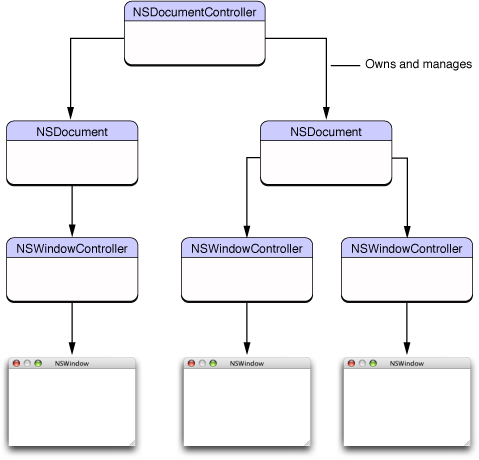
\includegraphics[scale=0.4]{Pictures/Chapter4/Diseinua/nsdocument.png}
\caption{Dokumentu arkitektura}
\label{nsdoc}
\end{center}
\end{figure}

\subsubsection{Ohiko atazak}
Lehen esan bezala, badaude programa hauetan oso ohikoak diren funtzionalitate batzuk, eta dokumentu arkitekturak lana asko errazten digu hauek inplementatzeko. \texttt{NSDocument}-en azpiklasean bi metodo inplementatu beharko dira:
\begin{itemize}
\item \texttt{-dataOfType:typeName error:aError}:

\texttt{NSData} motako objektu bat (\texttt{NSString} bat kodifikazioa espezifiko batekin, \textbf{UTF8} gure kasuan) itzuli behar du dokumentuaren edukiarekin fitxategi batean gordetzeko. \texttt{typeName} parametroarekin jakingo dugu zein den fitxategiaren formatua.

\item \texttt{-readFromData:data ofType:typeName error:aError}:

\texttt{NSData} motako objektu bat (data) eta fitxategiaren formatua jasotzen du. Bere eginkizuna zera da: edukia irakurtzea eta dokumentuko datu egiturak betetzea.
\end{itemize}

Erabilpen kasu hauen sekuentzia diagramak ez dira egingo: G01 - Fitxategia ireki, G02 - Script berria sortu eta G03 - Fitxategia gorde, Apple-en dokumentazioan\footnote{Apple-en dokumentazioko\cite{ap:dba} 29. orrialdean: \url{http://developer.apple.com/documentation/Cocoa/Conceptual/Documents/Documents.pdf}} aurkitu daitezkeelako, nahiz eta apur bat zahartuta egon (goian aipatutako metodoak ez dira erabiltzen, hauen ordez apur bat zaharragoak baina eginkizun berdina dutenak erabiltzen dira).

Sekuentzia diagramak ikusita, guk oso gutxi programatu beharko dugu (bi funtzio) fitxategiak ireki, itxi eta gordetzeko, kode asko aurreztuz (adibidez ez dugu fitxategia aukeratzeko panela maneiatu beharko edo dokumentuaren instantzia berria sortu beharko).

\subsubsection{Desegin/Berregin}
Aukera hauek inplementatzeko dokumentu arkitekturak ere lana asko erreztuko digu. \texttt{NSDocument}-ek \texttt{NSUndoManager} en instantzia bat dauka. Adibidez, aplikazioan lerro berri bat gehitzen dugunean, \texttt{NSUndoManager}-ean kontrako ekintza erregistratuko dugu, kasu honetan lerroa kentzea. Azken finean bi pila dauzka \texttt{NSUndoManager}-ek, bat desegiteko ekintzekin eta beste bat berregiteko ekintzekin. Desegitea aukeratzen dugunean, berregiteko pilan txertatuko da kontrako ekintza eta alderantziz. Menuko aukerak ere automatikoki kudeatuko dira guk ezer egin gabe.

\subsubsection{Dokumentuaren egoera}
Dokumentuan aldaketaren bat egin badugu, dokumentuaren aldaketa kontagailua inkrementatuko dugu. Kontagailu hau 0 ez bada, dokumentua zikin dagoela esango dugu, hau da, fitxategi sisteman dagoen fitxategia eta aplikazioan kargatuta dagoen dokumentua ez dira berdinak. Programa ixten saiatzen bagara, mezu bat agertuko zaigu zer egin nahi dugun galdetuz (gorde, ez gorde edo ezeztatu).

Aldaketaren bat desegiten badugu, kontagailua murriztuko da, eta fitxategia gordetzen badugu, kontagailuaren balioa 0 izango da berriz ere.

Aurreko kasuetan bezala, esfortzu gutxirekin (kode lerrorik gabe), funtzionalitate hau inplementatuta edukiko dugu.

\subsubsection{Informazio gehiago}
Atal honetan ikusi dugunez, erraztasun asko ematen dizkigu dokumentu arkitekturak, baina askoz gauza gehiago egiteko ere gai da. Informazio gehiago aurkitu daiteke Apple-ek eskaintzen duen dokumentazioan\cite{ap:dba}.

\subsection{Notifikazio bidezko komunikazioa}
Geroago sekuentzia diagrametan ikusiko denez, objektuen arteko zenbait komunikazioa notifikazio bidez egin dira, \textit{Observer} patroia jarraituz. Exekutatzen ari den aplikazio orok \textit{NSNotificationCenter} klasearen instatzia bat du, aplikazioaren edozein partetik atzigarria dena. Bertan notifikazioak \textbf{bidaliko} dira alde batetik, eta notifikazioen zain \textbf{erregistratuko} dira zenbait objektu. Erregistratzeko unea instantzia sortzerakoan da, eta bertan azalduko da zein notifikazioren zain erregistratu, noren notifikazioak jaso, etab. eta instantzia suntsitzean erregistratuta zegoena ezabatu behar da. Notifikazioa iristen direnean metodo konkretu bat exekutatuko du instantziak, metodo horien parametroa bakarra izanda: \textit{NSNotification} motako objektu bat bidaltzailearen informazioarekin.
 
Adibidez interfazean agertzen diren tauletan (\textit{NSTableView} klasekoak) erabiltzen da: erabiltzaileak lerro bat aukeratzen duenean notifikazioa bat bidaltzen da: NSTableViewSelectionDidChangeNotification izenekoa. \textit{ASSScriptController} klasean notifikazio horren zain geratu gara, eta iristen denean lehioaren goiko eremuetan aukeratutako lerroaren informazioa kargatuko da. Portaera hau \ref{notification}~Irudian azalduta agertzen da.
\begin{figure}[htp]
\begin{center}
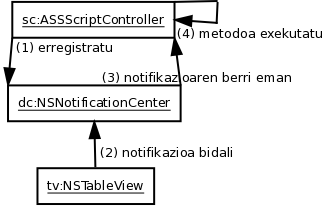
\includegraphics[scale=0.4]{Pictures/Chapter4/Diseinua/notification.png}
\caption{Notifikazio bidezko komunikazioa}
\label{notification}
\end{center}
\end{figure}

Guzti hau beste modu batean inplementatu daiteke, \textbf{delegate} izeneko loturen bidez, \ref{delegate}~Irudian ikus dezakegunez. Zenbait klaseek \textit{delegate} motako metodoak dituzte, eta hauek exekutatzeko klase horren instantziak lotuta egon behar dira beste klase baten instantziarekin, \textit{delegate} loturaren bidez Interface Builder-etik. Aurreko kasuan adibidez, \textit{NSTableView}-k badu horrelako metodo bat: tableViewSelectionDidChange, lehenago aipatu dugunaren gauza berdina egiten duena. Bien desberdintasuna hau da: Instantzia batek \textit{delegate} bidez beste instantzia batekin eduki dezake bakarrik lotura, eta notifikazio bidez instantzia batek bidali ditzake notifikazioak eta \textit{n} instantziek jaso ahal dute.
\begin{figure}[htp]
\begin{center}
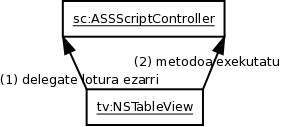
\includegraphics[scale=0.4]{Pictures/Chapter4/Diseinua/delegate.png}
\caption{Delegate bidezko komunikazioa}
\label{delegate}
\end{center}
\end{figure}

Beste gauza baterako erabili dira notifikazioak aplikazioan, adibidez G08 erabilpen kasuan, goiburuko bat ezabatzerakoan \textit{ASSScript} klaseak ezabatzen du dagokion datu egituratik, eta goiburuko editorearen kontrolatzaileak (\textit{ASSHeadersController}) jakin beharko du goiburukoak aldatu direla zerrenda berriro kargatzeko. Momentu honetan pentsa daiteke: "Zergatik ez egin zuzenean objektuen arteko mezu baten bidez, ASSScript-etik ASSHeadersController-era?", eta erantzuna sinplea da, ASSHeadersController-en instantzia bat ez da beti egongo, goiburukoen kudeaketarako lehioa ixterakoan instantzia suntsituko delako. Horrela, goiburukoak aldatzerakoan (goiburuko kudeatzailetik, edo adibidez Desegin/Berregin aukeretatik) notifikazioa bidaliko da, eta ASSHeadersController-en instantzia bat badago memorian notifikazioa jasotzerakoan zerbait egingo du. Ez badago instantziarik momentu horretan notifikazioa galduko da eta ez da ezer gertatuko.

Mota honetako komunikazioak aurrerago ikusiko ditugun sekuentzia diagrametan modu sinplifikatuan adierazi dira: beste objektuen arteko metodo bat izango balitz bezala, baina geziaren lerroa marra soil bat izan ordez marra eta puntuak tartekatzen dituena erabiliz.

\subsection{Sheet motako lehioak}
Aplikazioak zenbait lehio desberdin edukiko ditu. Lehio horietatik bat lehio nagusia izango da eta dokumentu bat irekita dagoen bitartean lehio hau irekita egon beharko da. Beste lehioak lagungarri bezala uler daitezke: lehio nagusiak informazio nagusia edukiko du (azptituluen lerroak hain zuzen ere), eta beste lehioak dokumentuko beste informazioa erakusteko (goiburukoak eta estiloak) edo laguntzaileak erakusteko erabiliko dira. Momentu batean lehio asko egon daitezeke irekita, eta hau ez da oso erosoa lan egiteko, gainera ez da beharrezkoa mota honetako aplikazio batean. Soluzio \textit{sheet} motako lehioak erabiltzea da, \ref{sheet}~Irudian ikus dezakegunez, lehio nagusitik \textit{zintzilikatuta} agertuko dira beste lehioak, eta itxi arte ez zaio lehio nagusiari kontrola itzuliko. Noski, modu honetan eginda, sheet motako lehio bakar bat irekita eduki ahal izango dugu, beraz arazoa konpondu dugu.
\begin{figure}[htp]
\begin{center}
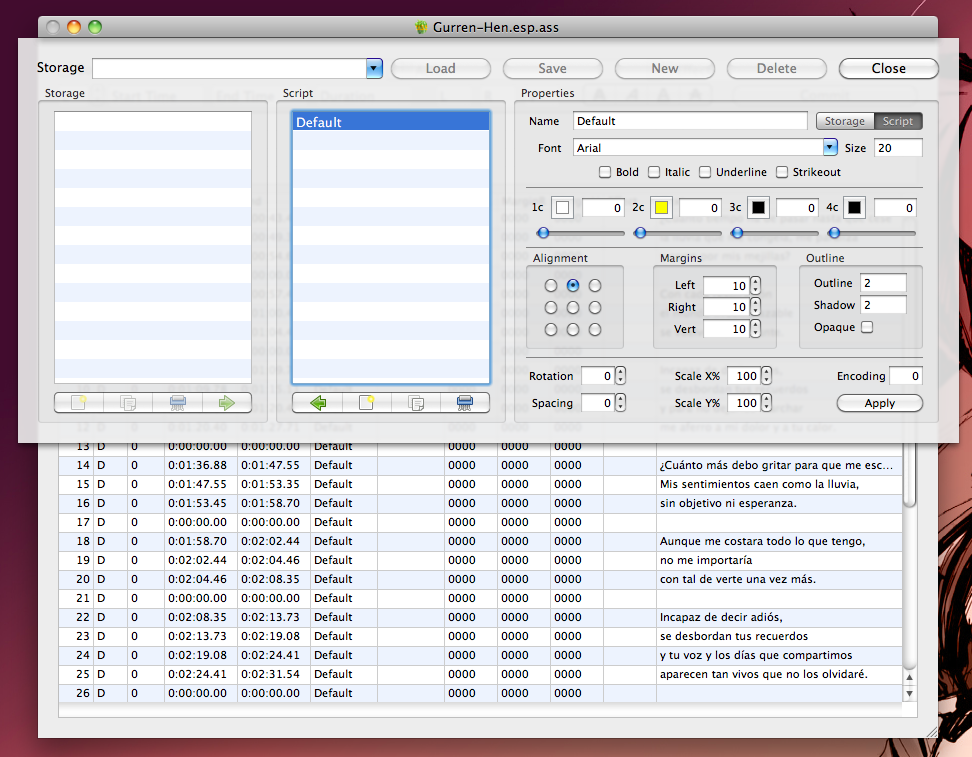
\includegraphics[scale=0.4]{Pictures/Chapter4/Diseinua/Sheet.png}
\caption{Sheet motako lehioaren adibidea}
\label{sheet}
\end{center}
\end{figure}
Mota honetako lehioak sortzea oso sinplea da. Lehenbizi lehioa diseinatu behar da beste lehio bat izango balitz bezala, eta lehioa erakutsi nahi dugunean \textbf{NSApplication} klasearen metodo baten bidez egiten da (\textbf{NSApp} \textit{NSApplication} klasearen instantzia bat da, exekuzioan dagoen aplikazio bakoitzak duena):
\texttt{[NSApp beginSheet:sheetWindow modalForWindow:mainWindow]}

\newpage
\subsection{Klase diagrama}

Lehenago aipatu den moduan, aplikazioa diseinatzeko orduan \textit{Model-View-Controller} patroia erabili da, beraz geroago erabiliko diren klaseak definitzerakoan 3 multzo horietan banatu dira, nahiz eta batzutan klase bat kategoria bat baino gehiagokoa izango den. Kontrakorik esaten ez bada, klase guztiak \textbf{NSObject} klasearen azpiklase dira. Hurrengo irudietan kurtsibaz agertzen diren klaseak ez ditugu guk inplementatu, Cocoa API-aren parte dira.

\subsubsection{Model klaseak}
ASS formatua da aplikazioak maneiatuko duen formatua, baita barne errepresentaziorako erabiliko duena, beraz \ref{kd-model}~Irudian ikus daitezke zeregin horretarako egin diren klaseak eta hauen erlazioak.
\begin{figure}[htp]
\begin{center}
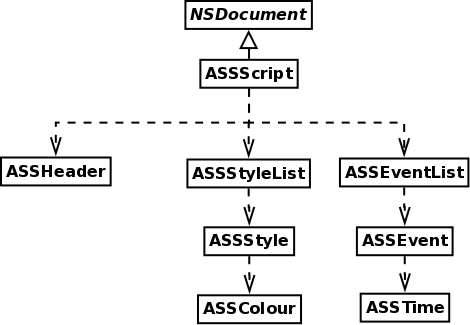
\includegraphics[scale=0.4]{Pictures/Chapter4/Diseinua/KD-Model.png}
\caption{Model klaseak}
\label{kd-model}
\end{center}
\end{figure}
\textit{ASSScript} da script oso bat errepresentatzen duen klasea, \ref{kd-model}~Irudian ikusten denez beste klase batzuen laguntzaz. Script baten edukia zenbait klaseetan banatu da, bertan agertzen diren elementuak identifikatuz eta hierarkia baten bidez errepresentatuz. \textit{ASSCript} \textbf{NSDocument} klasearen azpiklasea da, \textit{Document Based Applications} motako aplikazioetan agertu behar den klase bat, eta bertan datuez gain aplikazioaren kontrolerako metodoak ere badaude, adibidez fitxategia nola ireki, nola gorde, etab. Ondorioz esan dezakegu \textit{ASSScript} \textbf{Model} eta \textbf{Controller} motako klasea dela.

\subsubsection{View klaseak}
Interfazean erabiltzen diren klaseen azpiklaseak egin dira multzo honetan, \ref{kd-view}~Irudian ikus daitekeen moduan. Jatorrizko klaseek ez zuten nahi genuen funtzionamendua, beraz hauen azpiklaseetan zenbait metodo berridatzi dira. Adibidez \textit{ASSTranslationTextView} klasean \textbf{keydown:} metodoa berridatzi da, zenbait tekla zapaltzerakoan funtzionamendu espezifiko bat eduki dezan. Aipatu beharra dago \textit{Cocoa} ez dela software irekia, beraz ez dakigu zehatz mehatz zer egiten duen adibidez \textit{NSTextView} klaseak, beraz ez da oso erreza izan azpiklase hauek egitea.
\begin{figure}[htp]
\begin{center}
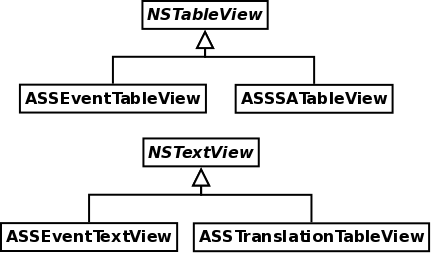
\includegraphics[scale=0.4]{Pictures/Chapter4/Diseinua/KD-View.png}
\caption{View klaseak}
\label{kd-view}
\end{center}
\end{figure}

\subsubsection{Controller klaseak}
\ref{kd-controller}~Irudian ikus daitezke Controller motako klaseak. Alde batetik \textit{NSWindowController} klasearen azpiklaseak dauzkagu, hauek direlarik aplikazioan aurkituko ditugun \textit{Controller} motako klase \textit{puruak}. Izenak dioen bezala, interfazean agertuko diren lehioen kontrolatzaileak izango dira hauek, interfazea datuekin lotuko dituztenak. Klase bakoitzak interfazeko lehio bat kontrolatuko du, ASSScript klasea ezik, lehio nagusiaz gain laguntzaileen lehio sinpleak ere kontrolatuko dituelako. Lehen aipatu den moduan, \textit{ASSScript} klasea \textit{Controller} motako ere bada, kasu honetan beste kontrolatzaileen kontrolatzailea hain zuzen. Irekita dugun dokumentu bakoitzeko \textit{ASSScript} instantzia bat edukiko dugu, eta honek gestionatuko ditu lehioak noiz eta nola ireki behar diren, etab.
\begin{figure}[htp]
\begin{center}
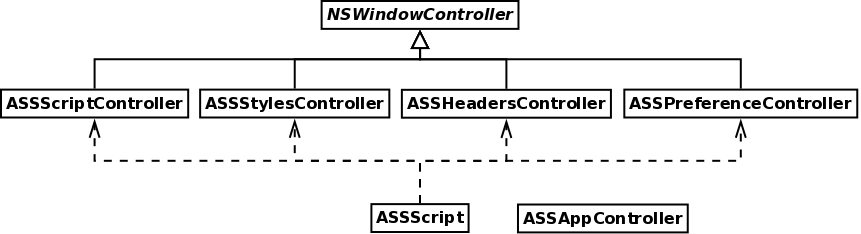
\includegraphics[scale=0.3]{Pictures/Chapter4/Diseinua/KD-Controller.png}
\caption{Controller klaseak}
\label{kd-controller}
\end{center}
\end{figure}
Bestalde, \textbf{AppController} klasea agertzen da \ref{kd-controller}~Irudian, daukan izenarekin pentsa dezakegu bere eginkizuna oso zabala eta konplexua dela, baina ez, kasu honetan defektuzko hobespenak ezartzea eta erabiltzaileak ezarri dituenak aktibatzea da.

\subsubsection{Bestelako klaseak}
Multzo honetan garapenerako lagungarriak izan diren klaseak dauzkagu. \ref{kd-others}~Irudian agertzen den klasea berezia da, bere izena soilik ikusita nabaritu daitekeena: \textbf{NSString+reverse}. NSString klasea Cocoa-k eskaintzen du zuzenean, eta izenak dioenez testu kateak errepesentatzen ditu. Kasu honetan, klase bat baino, Cocoa hizkeran \textbf{kategoria} bat dela esaten dan.
\begin{figure}[htp]
\begin{center}
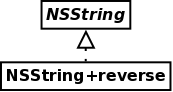
\includegraphics[scale=0.4]{Pictures/Chapter4/Diseinua/KD-Others.png}
\caption{Bestelako klaseak}
\label{kd-others}
\end{center}
\end{figure}
Beste lengoaia batzuetan, erabil dezakegun baina eraldatu ezin dugun klase bati funtzionalitate bat gehitu nahi diogunean (adibidez metodo berri bat gehitu), klase horren azpiklase bat sortzen dugu eta funtzionalitatea gehitzen diogu. Horretarako erabiltzen dira kategoriak Cocoa-n, adibidez \ref{kd-others}~Irudian NSString klaseari \textbf{reverse:} metodoa gehitu zaio, alderantzizkatutako karaktere katea itzultzen duena. Zein da honen abantaila: metodo hau erabili nahi badugu egin behar dugun bakarra \texttt{\#import "NSString+reverse.h"} erabili nahi dugun fitxategian gehitzea da, eta metodoa erabili ahal izango dugu \textit{NSString} motako objektuekin zuzenean.

\newpage
\subsection{Sekuentzia diagramak}
Atal honetan lehenago definitu diren erabilpen kasuen sekuentzia diagramak agertzen dira. Hauetako gutxi batzuk azalduko dira, besteen funtzionamendua ulertzea erraza delako behin batzuk azalduta egonda.

\subsubsection{G04 - Goiburukoak kudeatu}
Erabiltzaileak dagokion aukeran klik egiterakoan showHeadersManager mezua bidaliko zaio ASSScript-en instantziari. Honek lehio maneiatzailearen instantzia berri bat sortuko du, ASSHeadersController klasekoa, eta sortu berri duen instantzia hau lehio maneiatzaileen zerrendara gehituko du. ASSHeadersController-ek setDocument mezua jasoko du bere dokumentu bezala ASSScript instantzia ezartzeko. Azkenik, ASSHeadersController zenbait notifikazioren zain erregistratuko da.

\begin{figure}[htp]
\begin{center}
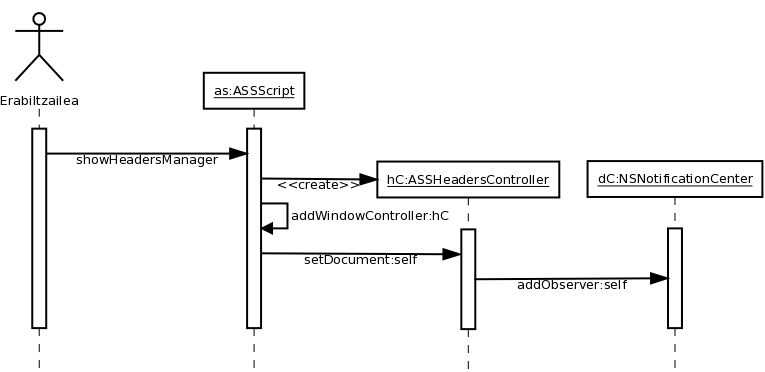
\includegraphics[scale=0.35]{Pictures/Chapter4/Diseinua/G04.png}
\caption{G04 - Goiburukoak kudeatu}
\label{g04d}
\end{center}
\end{figure}

\subsubsection{G05 - Goiburukoa sortu}
Erabiltzaileak botoian klik egiterakoan addHeader mezua bidaliko dio aurreko diagraman sortu den instantziari (Interface Builder-en bidez egin dugu lotura hau). ASSScript-i esan behar zaio goiburuko berri bat sartu behar dela (horretarako aurreko diagraman setDocument metodoaren bidez ASSScript-en instantzia gorde da). ASSScript-ek ez dauka goiburukoen zerrenda, bertan dagoen headers instantzian daude, ASSHeader klasekoa, beraz orain bai mezu baten bidez goiburuko berria zerrendan txertatuko da. Azkenik goiburuko kudeatzailean goiburukoen zerrenda eguneratu behar da, eta horretarako ASSScript-ek notifikazio bat bidaliko du, ASSHeadersController-en instantziak jasoko duena (aurreko diagraman erregistratu da).

\begin{figure}[htp]
\begin{center}
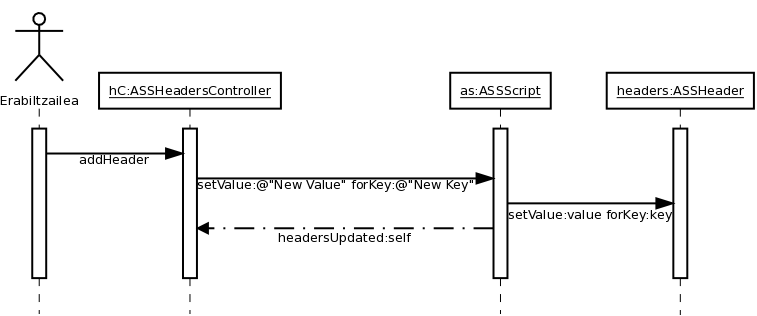
\includegraphics[scale=0.35]{Pictures/Chapter4/Diseinua/G05.png}
\caption{G05 - Goiburukoa sortu}
\label{g05d}
\end{center}
\end{figure}

\subsubsection{G06 - Goiburukoa aukeratu}
\begin{figure}[htp]
\begin{center}
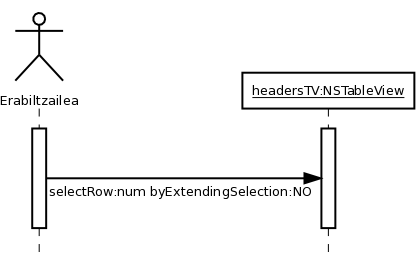
\includegraphics[scale=0.4]{Pictures/Chapter4/Diseinua/G06.png}
\caption{G06 - Goiburukoa aukeratu}
\label{g06d}
\end{center}
\end{figure}

\newpage
\subsubsection{G07 - Goiburukoa editatu}
\begin{figure}[htp]
\begin{center}
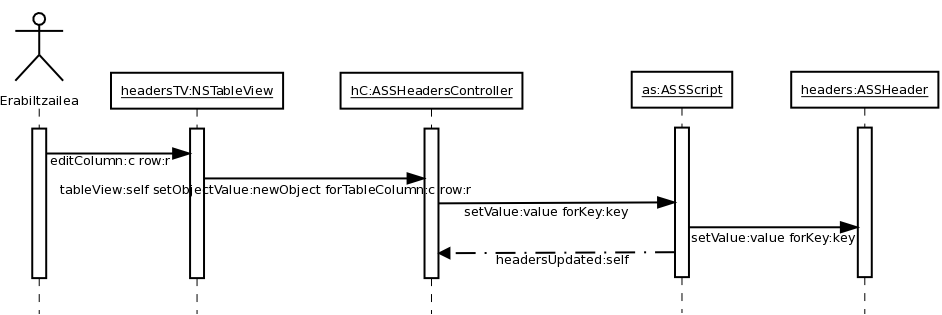
\includegraphics[scale=0.30]{Pictures/Chapter4/Diseinua/G07.png}
\caption{G07 - Goiburukoa editatu}
\label{g07d}
\end{center}
\end{figure}

\subsubsection{G08 - Goiburukoa ezabatu}
\begin{figure}[htp]
\begin{center}
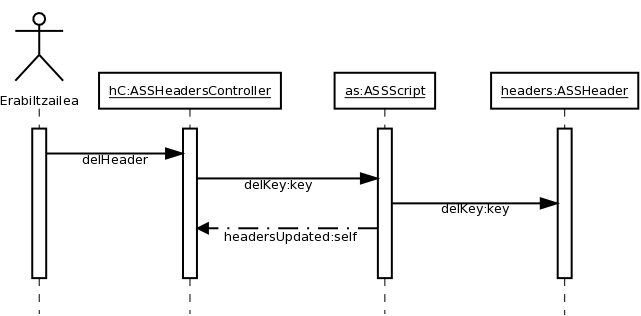
\includegraphics[scale=0.4]{Pictures/Chapter4/Diseinua/G08.png}
\caption{G08 - Goiburukoa ezabatu}
\label{g08d}
\end{center}
\end{figure}

\newpage
\subsubsection{G09 - Estiloak kudeatu}
\begin{figure}[htp]
\begin{center}
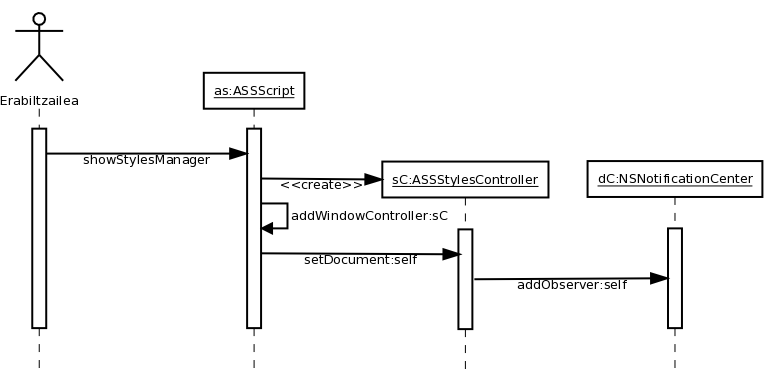
\includegraphics[scale=0.35]{Pictures/Chapter4/Diseinua/G09.png}
\caption{G09 - Estiloak kudeatu}
\label{g09d}
\end{center}
\end{figure}

\subsubsection{G10 - Estilo berria sortu}
\begin{figure}[htp]
\begin{center}
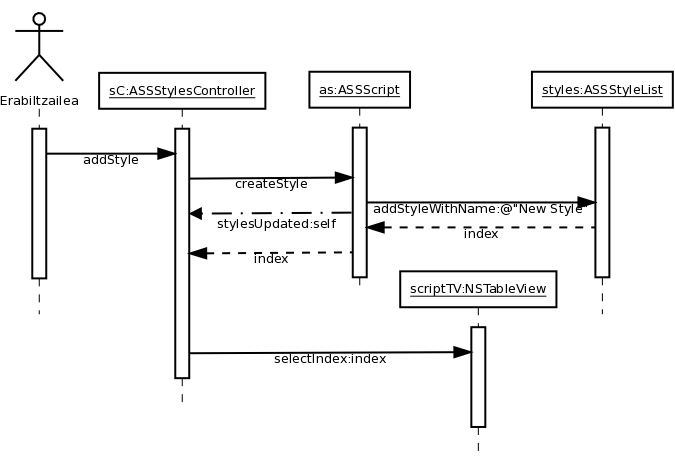
\includegraphics[scale=0.35]{Pictures/Chapter4/Diseinua/G10.png}
\caption{G10 - Estilo berria sortu}
\label{g10d}
\end{center}
\end{figure}

\newpage
\subsubsection{G11 - Estiloa aukeratu}
\begin{figure}[htp]
\begin{center}
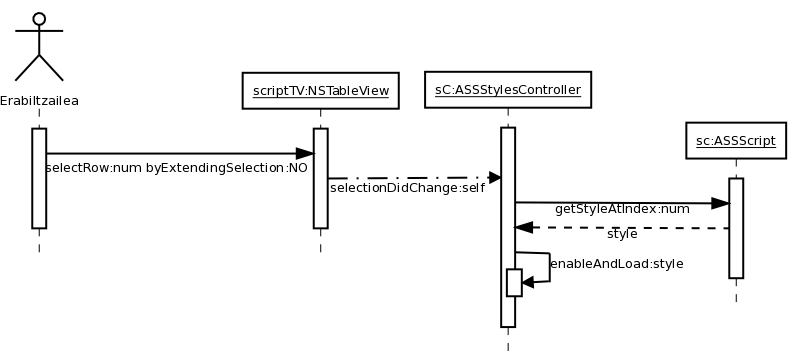
\includegraphics[scale=0.35]{Pictures/Chapter4/Diseinua/G11.png}
\caption{G11 - Estiloa aukeratu}
\label{g11d}
\end{center}
\end{figure}

\subsubsection{G12 - Estiloa editatu}
\begin{figure}[htp]
\begin{center}
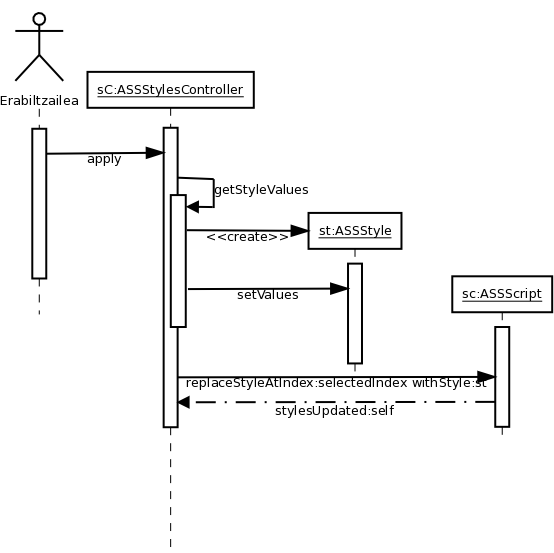
\includegraphics[scale=0.3]{Pictures/Chapter4/Diseinua/G12.png}
\caption{G12 - Estiloa editatu}
\label{g12d}
\end{center}
\end{figure}

\subsubsection{G13 - Estiloa kopiatu}
\begin{figure}[htp]
\begin{center}
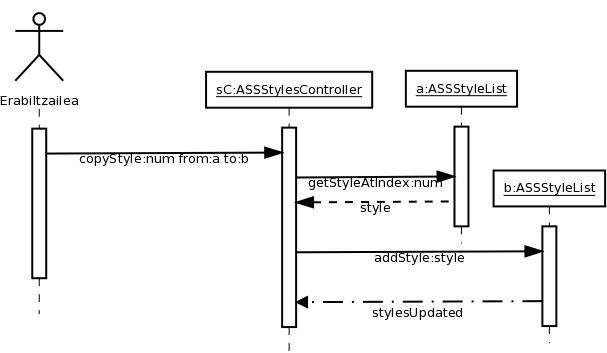
\includegraphics[scale=0.35]{Pictures/Chapter4/Diseinua/G13.png}
\caption{G13 - Estiloa kopiatu}
\label{g13d}
\end{center}
\end{figure}

\subsubsection{G14 - Estiloa ezabatu}
\begin{figure}[htp]
\begin{center}
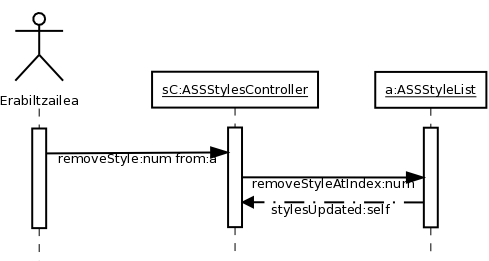
\includegraphics[scale=0.35]{Pictures/Chapter4/Diseinua/G14.png}
\caption{G14 - Estiloa ezabatu}
\label{g14d}
\end{center}
\end{figure}

\newpage
\subsubsection{S01 - Lerroak aukeratu}
Lerro zerrendan lerroren bat aukeratzerakoan selectRowIndexes metodoa bidaliko zaio ASSEventTableView-ren instantziari. Honek notifikazio bat bidaliko du, eta ASSScriptController egongo da honen zain. Lerro bakarra aukeratu bada, interfazean lerro horren datuak kargatu beharko dira, eta horretarako lerroa lortu beharko da getEventAtIndex metodoaren bidez. Azkenik interfazeko kontrolak aktibatu behar dira eta bertan kargatu behar dira lerroaren datuak.
\begin{figure}[htp]
\begin{center}
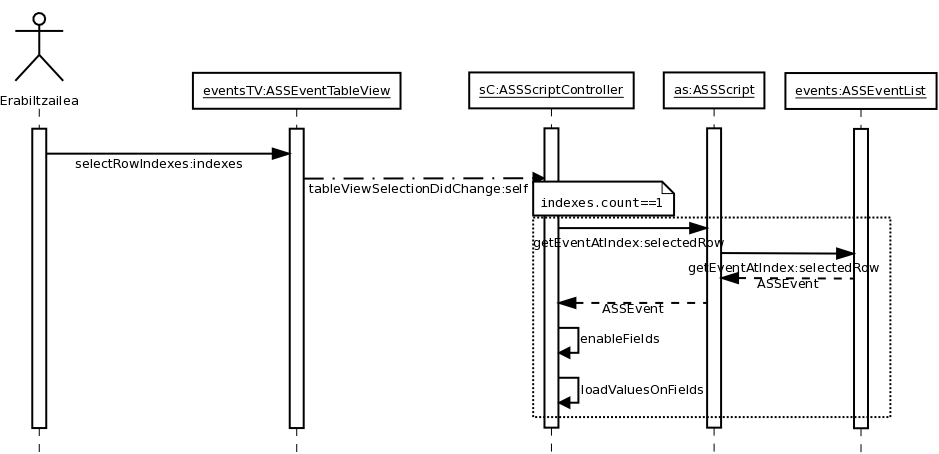
\includegraphics[scale=0.3]{Pictures/Chapter4/Diseinua/S01.png}
\caption{S01 - Lerroak aukeratu}
\label{s01d}
\end{center}
\end{figure}

\subsubsection{S02 - Lerroko eremua aldatu}
Lerroko eremuaren bat aldatzeko, interfazean aldatzeaz gain "Commit" botoia sakatu behar du erabiltzaileak, eta honen ondorioz commitEvent mezua bidaliko zaio ASSScriptController-en instantziari. Honek ASSEvent-en instantzia berri bat sortuko du eta interfazean agertzen diren datuak sartuko ditu bertan. Ondoren aurretik zegoen ASSEvent konkretua kendu behar da eta sortu berri duguna sartu behar da, replaceEventAtIndex metodoak egiten du hau, ASSScript-ek jasoko duena. ASSEventList-en events instantzia egin behar dira aldaketak, eta azkenik notifikazio bat bidali behar da interfazea datu berriekin eguneratzeko.
\begin{figure}[htp]
\begin{center}
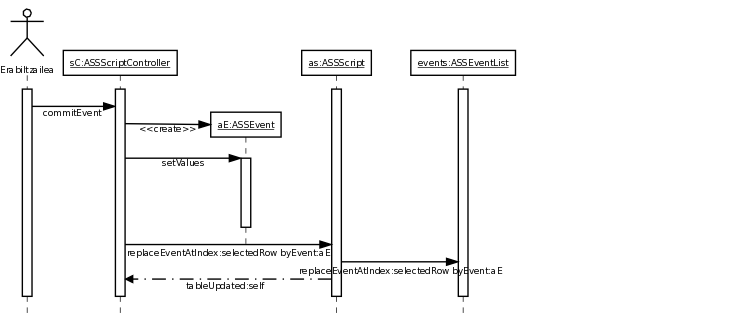
\includegraphics[scale=0.6]{Pictures/Chapter4/Diseinua/S02.png}
\caption{S02 - Lerroko eremua aldatu}
\label{s02d}
\end{center}
\end{figure}

\subsubsection{S03 - Lerroa gehitu}
\begin{figure}[htp]
\begin{center}
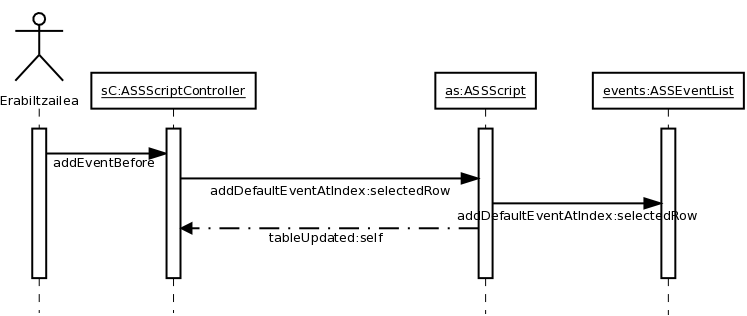
\includegraphics[scale=0.35]{Pictures/Chapter4/Diseinua/S03.png}
\caption{S03 - Lerroa gehitu}
\label{s03d}
\end{center}
\end{figure}

\newpage
\subsubsection{S04 - Lerroa kendu}
\begin{figure}[htp]
\begin{center}
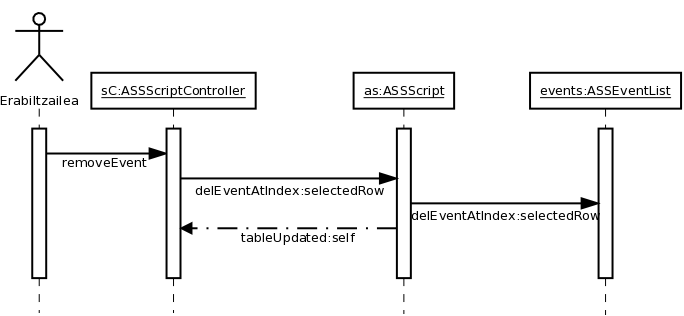
\includegraphics[scale=0.35]{Pictures/Chapter4/Diseinua/S04.png}
\caption{S04 - Lerroa kendu}
\label{s04d}
\end{center}
\end{figure}

\subsubsection{S05 - Lerroa bikoiztu}
\begin{figure}[htp]
\begin{center}
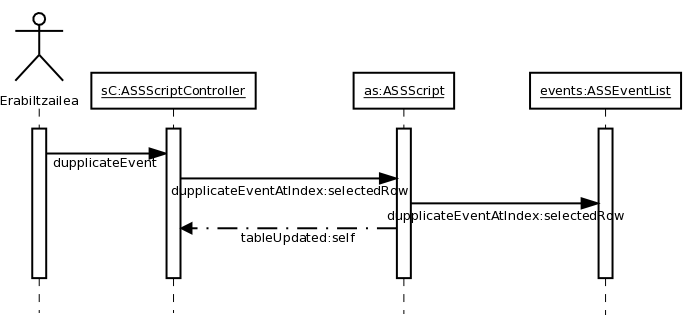
\includegraphics[scale=0.35]{Pictures/Chapter4/Diseinua/S05.png}
\caption{S05 - Lerroa bikoiztu}
\label{s05d}
\end{center}
\end{figure}

\newpage
\subsubsection{S06 - Lerroak desplazatu}
Lehenik sheet motako lehio bat sortu behar da, horretarako NSApp instantziari beginSheet metodoa bidaliz. Erabiltzaileak agertzen diren aukeretatik batzuk ezarriko ditu eta "Shift" botoia sakatuko du aukeratu duena aplikatzeko. "Shift" sakatzerakoan ASSScriptController-i iritsiko zaio shiftTimes mezua, baina aldaketak ASSScript-en instantzian egin behar dira, beraz interfazeko behar dugun informazioa hartuko du eta ASSScript-i bidaliko dio shiftTimes:direction forRows:rows affectedTimes:at time:t mezuaren bidez. Honek egin behar dituen aldaketak egiterakoan notifikazio bat bidaliko du interfazean eguneraketak egiteko.
\begin{figure}[htp]
\begin{center}
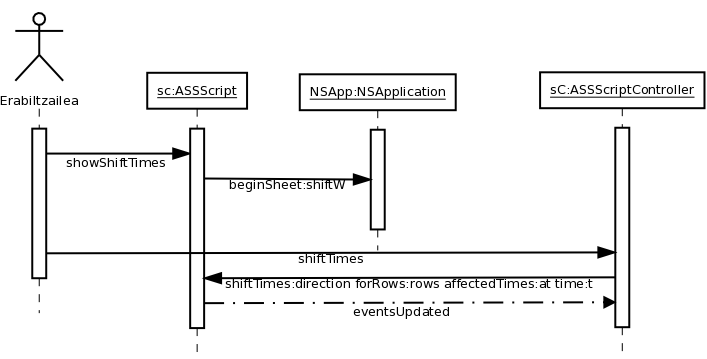
\includegraphics[scale=0.25]{Pictures/Chapter4/Diseinua/S06.png}
\caption{S06 - Lerroak desplazatu}
\label{s06d}
\end{center}
\end{figure}

\subsubsection{S07 - Lerroak batu}
\begin{figure}[htp]
\begin{center}
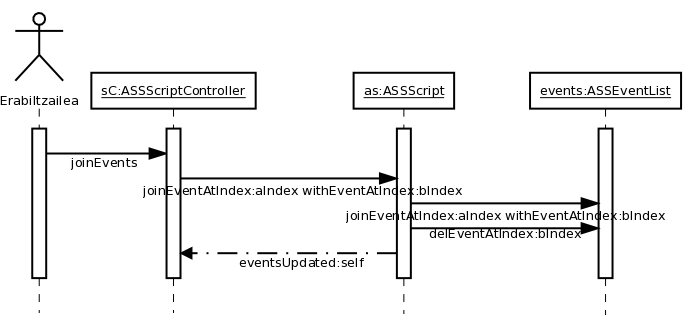
\includegraphics[scale=0.25]{Pictures/Chapter4/Diseinua/S07.png}
\caption{S07 - Lerroak batu}
\label{s07d}
\end{center}
\end{figure}

\newpage
\subsubsection{S08 - Estilo laguntzailea}
\begin{figure}[htp]
\begin{center}
\includegraphics[scale=0.4]{Pictures/Chapter4/Diseinua/S08.png}
\caption{S08 - Estilo laguntzailea}
\label{s08d}
\end{center}
\end{figure}

\newpage
\subsubsection{S09 - Itzulpen laguntzailea}
\begin{figure}[htp]
\begin{center}
\includegraphics[scale=0.4]{Pictures/Chapter4/Diseinua/S09.png}
\caption{S09 - Itzulpen laguntzailea}
\label{s09d}
\end{center}
\end{figure}

\newpage

\section{Inplementazioa}

\subsection{Kodearen kudeaketa}
Proiektuaren garapenerako bertsioen kontrolerako sistema (RCS\footnote{Revision Control System}) bat erabiltzea ezinbestekoa izan da, garapena ez delako konputagailu bakar batekin egingo, beraz kodea sinkronizatuta edukiko dugu hauetako software bat erabiliz.

SVN\footnote{Subversion} izan da garapenerako aukeratu den RCS-a, batez ere bi arrazoirengandik: ikasleak lehenago erabilia zuelako, horrela ikasketa prozesurik ez egoteko, eta erabili den garapen ingurunean zuzenean erabil daitekeelako.

Lehenago aipatu den moduan, \textit{Assembla.com}-eko zenbait zerbitzu erabili dira proiektuaren bizitzan zehar, eta webgune horrek SVN zerbitzaria eskaintzen duenez hori izan da erabili dena.

SVN-ri esker proiektuko kodea maneiatzea erosoa izan da, zenbait konputagailuetatik lana eginez inongo arazorik izan gabe. Aipatzekoa da ere, memoria hau SVN bidez ere kudeatu dela zerbitzari berdinean, \LaTeX{} fitxategiak azken finean testu fitxategiak direlako.

\subsection{Garapen ingurunea}
Programaren garapenerako eta lehenago aipatu denez, Apple-ek doan eskaintzen duen \textit{Xcode 3 Developer Tools} software konpilazioa erabili da. Bertan tresna asko agertzen dira baina guk ez ditugu guztiak erabili. Kodea idazteko, konpilatzeko, exekutatzeko eta arazteko \textbf{Xcode} erabili da.
\begin{figure}[htp]
\begin{center}
\includegraphics[scale=0.4]{Pictures/Chapter4/Inplementazioa/xcode.png}
\caption{Xcode IDE-a}
\label{xcode}
\end{center}
\end{figure}
\begin{figure}[htp]
\begin{center}
\includegraphics[scale=0.4]{Pictures/Chapter4/Inplementazioa/araztailea.png}
\caption{Xcode IDE-aren araztailea}
\label{debug}
\end{center}
\end{figure}
Barrutik UNIX inguruneetan ohikoak diren tresnak erabiltzen ditu, hala nola \textit{gcc}, \textit{gdb}, etab., baina dena interfaze grafikotik eginda, \ref{xcode} eta \ref{debug}~Irudietan ikusten denez.

Erabili den beste tresna garrantzitsua \textbf{Interface Builder} izan da, izenak esaten duen bezala interfaze grafikoak eraikitzeko tresna. Mac OS X sistemarako garapenean interfazeen sorkuntza desberdinduta dago kodetik. IB-rekin interfaze bat eraikitzerakoan, lehioen barruan elementuak sartuko ditugu: label-ak, testu-kutxak, taulak, etab. Objektuen instantziak ere sar ditzakegu ondoren hauekin loturak egiteko, horrela kodetik atzigarriak izateko interfazearen elementuak eta hauek erakusten duten informazioa.
\begin{figure}[htp]
\begin{center}
\includegraphics[scale=0.4]{Pictures/Chapter4/Inplementazioa/iblotura.png}
\caption{Interface Builder-en 'Action' motako lotura}
\label{ib1}
\end{center}
\end{figure}
\ref{ib1}~Irudian ikus dezakegu interfazeak edukiko duen lehio bat (ezkerrean), eta botoi batek objektu bati bidaliko dion mezua (lotura). Lotura \textit{File's Owner} ekin egiten da, \textit{NIB} bakoitzak horrelako bat eduki behar du, eta azken finean lehioa kontrolatuko duen klase baten instantzia izango da (kasu honetan \textit{ASSScriptController} klasekoa).

\begin{figure}[htp]
\begin{center}
\includegraphics[scale=0.4]{Pictures/Chapter4/Inplementazioa/iblotura2.png}
\caption{Interfaze builder-en 'Outlet' motako lotura}
\label{ib2}
\end{center}
\end{figure}

Aipatu denez, interfazeko datuak atzitu nahiko ditugu kodetik, beraz horrelako loturak ere egin beharko ditugu \ref{ib2}~Irudian ikus dezakeguna hain zuzen ere. Kodean aldagai bat izango dugu \textit{actorSATF} izenekoa irudian ikusten den \textit{textfield}-eko datuak irakurri eta idazteko.

IB-k informazioa \textit{XIB} edo \textit{NIB} formatuko fitxategietan gordetzen du, eta aplikazioa exekutatzerakoan kargatzen da hauen edukia. Gure kasuan zenbait fitxategi desberdin ditugu proiektuan: bat aplikazioaren menu barrarekin, beste bat lehio nagusia eta 'sheet' laguntzaileekin, beste bat estilo editorearen lehioarekin eta azkenik beste bat goiburuko editorearekin. \textit{XIB} eta \textit{NIB} fitxategien funtzioa berdina da baina bereizitasun bakarra dago bien artean, \textit{NIB} fitxategi bitarra da eta \textit{XIB} XML formatuan dago. Azken hau erabili dugu guk SVN-rekin lan egiteko gomendagarriagoak direlako testu fitxategiak.

\subsection{Erabiltzailearen datuak}
Programan exekuzio batetik bestera gorde behar diren datuak dauzkagu, beraz nonbait gorde behar ditugu fitxategietan. Horretarako aplikazioa exekutatzen ari den erabiltzailearen \textit{HOME} katalogoaren barruan gordeko dira datuak, konkretuki \textbf{/Users/erab/Library/} katalogoren barruan.

\subsubsection{Estilo biltegiak}
Kasu honetan, estiloak ASS formatuan bezala gordetzen dira /Users/erab/ Library/Application Support/GrosoSub/styles/ katalogo barruko fitxategi desberdinetan. \textbf{Application Support} katalogoa horretarako erabiltzen dute aplikazio guztiek, mota desberdinetako eta programak maneiatuko dituen datuak gordetzeko. Katalogoa ez bada existitzen programak sortuko du bertan zerbait gordeko duen lehenengo aldian.

\subsubsection{Hobespenak}
Aurrekoarekin alderatuta, preferentzien kontua desberdina da, aplikazio gehienetan ohikoa den funtzio bat denez beste forma batean gorde eta kudeatzen delako. XML formatuko fitxategi batean gordetzen dira preferentziak, /Users/erab/Library/Preferences/com.perryranch.grososub.plist hain zuzen ere (\textit{perryranch} agertzen da proiektuan ezarri den asmatutako enpresaren izena delako). Hobespenak maneiatzeko oso kode gutxi idatzi behar izan da, bakar bakarrik zeintzuk diren preferentzien defektuzko balioak. Erabiltzaileak ezarri dituen balioak hasieran kargatzeko eta programa ixtean gordetzeko Inteface Builder bidez egiten da, \textit{Cocoa bindings} izeneko teknika erabiliz, lehen ikusi dugun modu berdintsuan loturak ezarriz. \ref{prefs}~Irudian ikus daiteke aplikazioaren preferentzia lehioa.
\begin{figure}[htp]
\begin{center}
\includegraphics[scale=0.6]{Pictures/Chapter4/Inplementazioa/prefs.png}
\caption{Aplikazioaren preferentzia lehioa}
\label{prefs}
\end{center}
\end{figure}

Erabiltzaileak ezartzen dituen balioak aplikazioaren edozein partetik atzigarriak dira.

\subsection{Eguneraketa automatikoak}
Aplikazioaren eskakizunetan eguneraketa automatikoen kontua aipatzen da, eta horretarako Mac OS sisteman oso erabilia den \textit{framework} bat erabili da: \textbf{Sparkle\footnote{\url{http://sparkle.andymatuschak.org/}}}. Honetarako ere ez dugu kode lerro bakar bat ere idatzi behar izan, beharrezkoa izan den bakarra framework-aren webgunean azaltzen dituzten loturak Interface Builder-en egitea izan da.

Eguneraketen funtzionamendua erraza da: AppCast\footnote{\url{http://connectedflow.com/appcasting/}} formatua jarraitzen duen XML fitxategi bat atzigarri eduki behar dugu internet-en, baita aplikazioaren bertsio desberdinak eta hauen arteko informazioa ere (\textit{ChangeLog}). Horrela konfiguratzen badugu, aplikazioak noizbehinka begiratuko du ea eguneraketarik dagoen, eta horrela bada erabiltzaileari jakinaraziko dio. Honek baiztapena emango du eguneraketa gauzatzeko edo ez, geroagorako utziz edo bertsio konkretu hori ahaztuz.

Bestalde, eta \ref{prefs}~Irudian ikusten den bezala, eguneraketak egiterakoan sistemaren informazioa bidali daiteke (sistemaren bertsioa, hizkuntza, prozesadorea, etab.), garatzaileak ikus dezan zein motako sistemetan exekutatzen den aplikazioa. Bidaltzen den informazioa guztiz anonimoa da eta erabiltzailea ez dago batere behartuta informazio hau bidaltzera. Lehen eguneraketa egiterakoan honen inguruan galdetuko zaio erabiltzaileari eta bidaliko den informazioa ikusi ahal izango du.

Azkenik, erabiltzaileak nahi duenean begiratu dezake ea eguneraketarik dagoen menu-an agertzen den aukera batetik, eta prozesua aipatu dugun berdina izango litzateke.

\subsection{Exekutagarriaren sorkuntza}
Mac OS X sistema eragilea hiru arkitektura desberdinetan erabili daiteke. Alde batetik \textbf{X86} 32 eta 64 biteko makinetan, eta bestetik gero eta gutxiago erabiltzen diren \textbf{PPC} makinetan (32 eta 64 bitekoak hauek ere). Sistema eragilearen azkenengo bertsioan (10.6) PPC arkitektura kendu dute, X86 bakarrik geratuz, baina guk gure aplikazioa PPC makinetarako ere eskaini nahi dugu. Horretarako Xcode-ko proiektuan, SDK-ren 10.5 bertsioa aukeratu dugu, eta exekutagarri \textit{Unibertsala} sortzeko esan dugu, hau da, PPC eta X86 arkitekturetarako kode bitarra sortuko dugu aplikazioa konpilatzerakoan. Noski, aplikazioaren tamaina handiago izango da, baina hala ere 3 MiB inguru okupatzen ditu guztira.

Eskakizunetan aipatzen zen aplikazioa instalatzeko erraza izan behar zela, erabiltzaileak konpilatu behar ez izateko. Aplikazioa konpilatzerakoan, .app fitxategi batekin aurkituko gara. Nahiz eta sistemak fitxategi bezala ikusi, benetan katalogo bat da, eta barruan beharrezkoak diren gauza guztiak ditu: exekutagarria (arkitektura desberdinetarako), framework-ak, erabiltzen diren irudiak, ikonoak, itzulpena, etab.

Instalatzeko orduan programa gehienak instalatzen diren moduan egiten da, .app \textit{fitxategi} hori zuzenean \textbf{/Applications/} sistemako katalogora kopiatuz. Sisteman ohikoa den moduan, .app fitxategia \textbf{DMG}\footnote{\url{http://en.wikipedia.org/wiki/Apple_Disk_Image}} baten barruan sartu da. Aplikazioa sistematik ezabatzea ere erraza da, /Applications/ katalogotik ezabatuz nahikoa baita.

\section{Probak}
Softwarearen edozein garapen prozesutan logikoa denez, garatzen dena probatu egin behar da bere funtzionamendua egokia den jakiteko. Aplikazioaren izaera dela eta bi motako probak gauzatu dira.

\subsection{Proba unitarioak}
Aplikazioaren garapenaren hasieran, ASS formatua maneiatzeko beharrezkoa inplementatu zen. Gogoratu beharra dago aplikazioaren formatu 'natiboa' ASS dela, nahiz eta SRT formatuarekin ere lan egin daitekeen, SRT ASS-ren azpimultzo bezala ulertu daitekeelako, beraz aplikazioak barrutik ASS formatuarekin lan egingo du.

Inplementatu ziren klaseak eta hauen metodoak probatzeko proba unitarioak erabili dira, horrela zerbait aldatzean eta probak ondo diseinatuta badaude, probak berriro exekuta daitezke ikusteko ea zerbait apurtu dugun azken aldaketekin.

\subsubsection{SenTestingKit}
Xcode IDE-ak badauka proba unitarioentzako framework bat, SenTestintKit izenekoa. Hasieran Sen:te\footnote{\url{http://www.sente.ch/software/ocunit/}}-k garatu zuen OCUnit izenarekin, baina Xcode 2.1 bertsiotik aurrera Apple-ek eskaintzen duen software konpilazioaren barruan dago izen berriarekin.

Probatu nahi izan dugun klase bakoitzeko beste klase bat sortu dugu, \textit{SenTestCase} klasearen azpliklase direnak. Bertan egin nahi dugun test unitario bakoitzeko metodo bat jarri dugu, horien barruan probatu nahi duguna exekutatuz eta horren emaitza espero genuenarekin konparatuz, SenTestintKit-ek eskaintzen dituen \textbf{Assert} motako funtzioak erabiliz. Hona hemen test baten adibidea:

\begin{verbatimtab}[8]
- (void) testCompare
{
	ASSTime *t1 = [[ASSTime alloc]
			initWithString:@"1:44:03.88"];
	ASSTime *t2 = [[ASSTime alloc]
			initWithString:@"1:44:03.88"];
	ASSTime *t3 = [[ASSTime alloc]
			initWithString:@"1:44:06.88"];
	
	STAssertTrue([t1 compare:t2] == NSOrderedSame,
			@"This should be the same");
	STAssertTrue([t1 compare:t3] == NSOrderedAscending,
			@"t1 should be less than t3");
	STAssertTrue([t3 compare:t2] == NSOrderedDescending,
			@"t3 should be greater than t2");
}
\end{verbatimtab}

ASSTime klasearen hiru instantzia definitzen dira (t1, t2 eta t3), eta ondoren hiru gauza probatzen dira: t1 == t2, t1 $>$ t3 eta t3 $<$ t2. Test horietako bat ez bada betetzen, kodean jarri dugun mezua agertuko da interfazean eta errore bezala markatuko ditu lerroak, jakiteko zein izan den gaizki funtzionatzen duena.

\ref{ocunit}~Irudian ikus daiteke diseinatu diren proba unitario guztiak pasatzen direla arazorik gabe.
\begin{figure}[htp]
\begin{center}
\includegraphics[scale=0.6]{Pictures/Chapter4/Probak/ocunit.png}
\caption{Proba unitarioen exekuzioa}
\label{ocunit}
\end{center}
\end{figure}

Oraingo honetan ere, Apple-ek eskaintzen duen dokumentazioan\cite{ap:ocu} honi buruzko informazio mordoa aurkituko dugu.

\subsubsection{Egin diren probak}
\ref{ocunit}~Irudian ikus dezakegunez 22 proba unitario egin dira guztira honako klaseen funtzionamendu egokia bermatzeko:
\begin{itemize}
	\item ASSColour: \begin{itemize}
		\item Defektuzko balioa espero zena.
		\item Balio maximoa onartzen du.
		\item Ausazko balioa ondo jaso eta itzuli.
	\end{itemize}
	\item ASSEventList: \begin{itemize}
		\item Lista sortzerakoan item bakarra listan.
		\item Txertaketa, ezabaketa eta aldaketen eraginak zuzenak.
		\item Karaktere kate batetik datuak ondo jasotzen dira.
	\end{itemize}
	\item ASSEvent: \begin{itemize}
		\item Defektuzko balioa espero zena.
		\item Karaktere kate batetik datuak ondo jasotzen dira.
		\item Bi ASSEvent-en arteko 'join'-a ondo egiten da.
	\end{itemize}
	\item ASSHeader: \begin{itemize}
		\item Defektuzko balioa espero zena.
		\item Karaktere kate batetik datuak ondo jasotzen dira.
		\item Txertaketa, ezabaketa eta aldaketen eraginak zuzenak.
	\end{itemize}
	\item ASSStyleList: \begin{itemize}
		\item Lista sortzerakoan item bakarra listan.
		\item Karaktere kate batetik datuak ondo jasotzen dira.
	\end{itemize}
	\item ASSStyle: \begin{itemize}
		\item Defektuzko balioa espero zena.
		\item Ausazko ASSStyle bat jaso eta itzuli.
		\item Estiloetan agertzen diren balio boolearrak ondo errepresentatuta irteeran. 
	\end{itemize}
	\item ASSTime: \begin{itemize}
		\item Defektuzko balioa espero zena.
		\item Irteerako karaktere katea ondo sortzen du.
		\item Karaktere kate batetik datuak ondo jasotzen dira.
		\item Karaktere kate batekin zuzenean hasieratu daiteke.
	\end{itemize}
\end{itemize}

\subsection{Proba ez unitarioak}
Nahiz eta proba unitarioak oso ondo egon garapenean zehar behin eta berriz exekutatu ahal ditugulako programaren portaera zuzena dela egiaztatzeko, ezin dira programa osoa probatzeko erabili, adibidez, nola probatu interfaze grafikoa proba unitarioen bidez? SenTestingKit-ek behintzat ez du horrelakorik eskaintzen.

Beraz, aplikazioaren funtzionamendua egiaztatzeko modu bakarra aplikazioa erabiltzea da gauzak ondo dabiltzan edo ez ikusiz. Lana ez da makala, egoera eta ekintza konbinaketa handia delako eta seguraski arazoren bat ez dugu aurkituko. Dena den, proba prozesu hau erraztearren proiektuaren kanpoko zenbait pertsonen laguntza egon da, garapenean zehar aplikazioa erabili izan dutenak eta erroreak aurkitzerakoan komunikatu dituztenak.

Arazo \textit{arraroak} aurkitu direnean Xcode-k eskaintzen duen araztailea erabili da, programaren funtzionamendua pausoz pauso aztertuz errorea aurkitu arte.

\section{Kudeaketa}

\subsection{Jarraipen bilerak}
Proiektuaren garapenean zenbait bilera egin dira irakasle eta ikaslearen artean. Gehienak presentzialak izan dira, irakaslearen fakultateko bulegoan, baina ikaslea udan Donostian ez dagoenez, posta elektronikoz egin behar izan dira batzuk.

Bilera hauek lana pixkanaka planifikatzeko eta ikasleak izan dituen zalantzak argitzeko izan dira gehienbat. Hauek dira egin diren bilerak eta bertan tratatu dena:

\begin{enumerate}
	\item Bilera: \textit{2008. urteko Urriak 22}\\
		Proiektua planteatu zaio irakasleari eta honek onartu ondoren \textbf{proiekges} plataforman erregistratuko du ikasleak emandako proiektuaren deskribapenarekin.
	\item Bilera: \textit{2008. urteko Azaroak 3}\\
		Landu beharreko memoriaren edukien zehaztapena.
	\item Bilera: \textit{2008. urteko Abenduak 10}\\
		Otsaileko azterketak direla eta, proiektuaren garapena eteten da hauek amaitu arte.
	\item Bilera: \textit{2009. urteko Otsailak 11}\\
		Behin azterketak amaituta, proiektuarekin jarraitu behar da. Oraingoan Aurrekarien analisia egin behar da.
	\item Bilera: \textit{2009. urteko Otsailak 25}\\
		Aurrekarien analisia ondo egin da, beraz PHD-arekin jarraitu beharra dago.
	\item Bilera: \textit{2009. urteko Martxoak 12}\\
		PHD ondo dago, beraz Softwarearen garapenerako prozesu bateratuarekin hasi beharra dago. Eskakizunen bilketa egitea esleitu da oraingoan.
	\item Bilera: \textit{2009. urteko Martxoak 19}\\
		Lehenago pasatu den modu berdinean, proiektua momentuz geldituta geratzen da. Geldituta dagoen bitartean Ekaineko azterketak iritsi egiten dira eta hauek amaitzerakoan jarraituko da.	
	\item Bilera: \textit{2009. urteko Uztailak 3}\\
		Behin azterketak amaituta, lehenengo iterazioarekin hasten gara. Iterazio hau laburrena da, baina bertan zenbait gauza daude egiteko: analisia, diseinua, inplementazioa eta probak.
	\item Bilera: \textit{2009. urteko Uztailak 17}\\
		Lehenengo iterazioa amaituta dago, beraz 2. iterazioarekin hasiko gara. Honez gain lehengo iterazioan egin duguna dokumentatzen hasteko ordua da.
	\item Bilera: \textit{2009. urteko Uztailak 31}\\
		Garapenari buruzko zenbait duda argitu dira oraingoan, batez ere diseinuko sekuentzia diagramekin. Bigarren iterazioarekin jarraitu beharra dago.
	\item Bilera: \textit{2009. urteko Abuztuak 10}\\
		Zenbait arazo pertsonalengatik proiektuarekin jarraitzea ezinezkoa da momentuz, eta Irailean ezin izango da aurkeztu. Informatu ondoren hurrengo urtean \textit{matrikula erlaxatua} egiteko aukera hartuko da, horrela ikaslea Ingeniaritza Informatikoko bigarren zikloarekin hasi ahal izango da eta bitartean proiektua amaitu egingo du.
	\item Bilera: \textit{2009. urteko Irailak 2}\\
		Bigarren iterazioa amaitutzat ematen da eta hirugarren eta azkenengoarekin hasi beharra dago. Bertan egingo dena planifikatu da bilera honetan.
	\item Bilera: \textit{2009. urteko Urriak 2}\\
		Proiektuaren egoera egiteko bideo bat grabatu da non programaren funtzionamendua erakusten den. Bideoa ikusi egin da bileran eta konpontzeko zeuden gauzak apuntatu dira. Hurrengo asteetan hauek konponduko dira eta hirugarren iterazioarekin jarraituko da.
	\item Bilera: \textit{2009. urteko Urriak 27}\\
		Hirugarren iterazioarekin lanean jarraitzen du ikasleak, proiektua amaitzeko falta dena ikusteko egin da bilera hau.
	\item Bilera: \textit{2009. urteko Abenduak 9}\\
		Berriro ere zenbait arazo direla eta, proiektuarekin ezin da jarraitu. Honez gain Otsaileko azterketak direla eta hauek amaitu arte ezin izango da aurrera jarraitu.
	\item Bilera: \textit{2010. urteko Urtarrilak 31}\\
		Azkenean hirugarren iterazioarekin jarraitu ahal izan da, eta proiektuaren garapen fasea amaitu egin da. Dokumentazioa amaitu beharra dago eta dena entregatzeko prestatu behar da. Denbora oso justua da momentu honetan baina saiakera egin beharra dago.
	\item Bilera: \textit{2009. urteko Otsailak 12}\\ Dokumentazioa entragatu zaio irakasleari honek zuzendu ahal izateko. Bestalde bideoa, CD-a  eta aurkezpena prestatu behar dira.
\end{enumerate}

\subsection{Egoera txostenak}
Egin den iterazio bakoitza amaitzerakoan hurrengo iterazioa planifikatzeari ekin behar zaio, horretarako amaitu berri dena aztertuz eta ondorioak ateraz ondoren erabakiak hartzeko. Azkenengo iterazioa amaitzerakoan ez da egoera txostenik egin, eta horren ordez hurrengo atal batean aztertu da proiektuaren egoera globala.

\subsubsection{Lehenengo iterazioa}
Iterazio hau estimatutako denboran egin da, egun bat soberan izanda amaieran. Esan beharra dago iterazio hau sinpleena eta laburrena dela, baina momentuz badirudi dena ondo joaten ari dela, beraz ez da planifikazioan ezer aldatu behar eta bigarren iteraziorekin asteko ordua da.

Nahiz eta memoriaren garapena proiektuaren amaierarako planifikatuta egon, hasiko den bigarren iterazioarekin batera egiten joango da. Zenbait atala egiten joan daitezke, eta horrela lana pixkanaka eginez eramangarriago izango da. Iterazio berria bihar bertan hasiko da, Uztailak 17 eta Abuztuak 8-rako amaituta egotea espero da.

\subsubsection{Bigarren iterazioa}
Oraingoan gauzak ez dira planifikatu diren bezala joan, zenbait arazorengandik proiektua alde batera utzi behar izan delako eta ia hilabete bat beranduago amaitu da, Iralaren 2-an hain zuzen ere. Aurrera jarraitu ezin zela ikusi zenean, proiektuaren amaiera data berriro planifikatuko da, eta denborarik ez dagoenez 2009. urteko Irailean entregatzeko, 2010. urteko Otsailerarte atzeratuko da.

Nahiz eta atzerapenekin ibili, iterazio honetan egin beharreko egin da, eta aurreko iterazioan egin diren gauzak dokumentatu daude memorian. Programari begira, orain arte eginda dagoena funtzionatu egiten du eta hasieran zehaztutakoari jarraitzen dio.

Lehen bait lehen hirugarren iterazioarekin hasi beharra dago, eta estimazio berriak eginez Abenduaren erdialdera amaituta egon beharko litzateke, ondoren falta diren gauzak amaitzeko (memoria, CD-a, aurkezpena, etab.), horrela Urtarrilaren erdialderako proiektua guztiz amaituta egoteko.

Aurrekoan bezala, bigarren iterazio honetan egindakoa dokumentatzen hasiko gara memorian sartuz beharrezkoa dena, eta horrela poliki-poliki dokumentua osatzen joango gara.

\subsection{Proiektuan zehar egon diren arazo eta atzerapenak}
Jarraipen bileretan ikus daitekeenez, proiektuan zenbait atzerapen egon dira. Hasieran 2009. urteko Iraileko deialdirako proiektua aurkeztea pentsatu zen, horrela udan egin ahal izateko, kurtsoan zehar ikasleak lan zama handia zuelako ikasketekin. Proiektua ondo zihoan, baina zenbait arazok eten egin zuten Abuztuan.

Momentu horretan irtenbide bat bilatu behar izan zen, honelako kasuetarako fakultateak eskaintzen duen \textit{matrikula erlaxatua} hain zuzen ere. Ikasleak Sistemen Informatikan Ingeniari Teknikotik bakarrik proiektua du faltan, eta bere intentzioa Ingeniaritza Informatikoko bigarren zikloa egitea da, beraz hurrengo ikasturtean bigarren zikloko zenbait irakasgai izango ditu eta proiektua amaitu beharko du 2010. urteko Otsailerako.

Berriro ere dena ondo joaten ari zenean, arazoak berriro ere etorri ziren eta lana berriro birplanifikatu egin behar izan zen, azkenean proiektua amaituz baina soberan denbora oso gutxi izanda.

Arazo pertsonalez gain, nire ustez arazo larriena hau izan da: garrantzi gehiago eman zaie matrikulatutako irakasgaie proiektuari baino, eta denbora gehiago erabili da hauetarako, adibidez beharrezkoak (baina lagungarriak) diren zenbait azterketa partzial eginez. Orain ikusirik nola joan den proiektuaren azken fase hau ikus daiteke garrantzitsuago dela proiektua amaitzea beste irakasgaiak gaindetzea baino, proiektua ez bada gainditzen ezingo delako irakasgai horietan matrikula egin.

Dena den horrelako proiektuetan gerta daiteke zenbait arazo sortzea eta proiektua behin eta berriz atzeratzea, eta horrelako kasuetan zer egin behar den ikasteko ondo etorri da esperientzia hau.

\subsection{Amaierako ondorioak}
Hasieran, \textit{Proiektuaren Helburu Dokumentuan} estimazio batzuk egin ziren, bai esfortzuarenak baita iraupenarenak ere. Aurreko ataletan ikusi dugunez zenbait atzerapen egon dira, beraz iraupena nahi genuena baino askoz gehiago luzatu da. Ikus ditzagun bietan egon diren aldaketak.

\subsubsection{Benetako esfortzua}
\ref{benetako-esfortzua}~Taulan ikus dezakegu zein izan zen bere momentua estimatutako eta proiektua amaitzerakoan egin den benetako esfortzua.

\begin{longtable}{|l|l|l|r|}
\hline
\grey \textbf{Ataza} & \grey \textbf{Estimazioa} & \grey \textbf{Benetakoa} & \grey \textbf{Aldea}\\
\hline
\endhead
\hline
\caption{\label{benetako-esfortzua}Estimatuko esfortzua vs. Benetako esfortzua}
\endfoot
\bblue Kudeaketa & \bblue 30 & \bblue 26 & \bblue \%-13,33 \\
\hline
\blue \hspace{1em}Bilerak & \blue 25 & \blue 21 & \blue \%-16,00 \\
\hline
\hspace{2em}Ohiko bilerak & 20 & 17 & \%-15,00 \\
\hline
\hspace{2em}Aurrerapen bilerak & 5 & 4 & \%-20,00 \\
\hline
\blue \hspace{1em}Artxiboaren kudeaketa & \blue 5 & \blue 5 & \blue \%0,00 \\
\hline
\bblue Planifikazioa & \bblue 10 & \bblue 17 & \bblue \%+70,00 \\
\hline
\blue \hspace{1em}PHD egin & \blue 7 & \blue 12 & \blue \%+71,43 \\
\hline
\blue \hspace{1em}Iterazio berriaren planifikazioa & \blue 3 & \blue 5 & \blue \%+66,67 \\
\hline
\bblue Garapena & \bblue 130 & \bblue 167 & \bblue \%+28,46 \\
\hline
\blue \hspace{1em}Eskakizunen bilketa & \blue 10 & \blue 7 & \blue \%-30,00 \\
\hline
\blue \hspace{1em}Analisia & \blue 15 & \blue 20 & \blue \%+33,33 \\
\hline
\blue \hspace{1em}Diseinua & \blue 40 & \blue 45 & \blue \%+12,50 \\
\hline
\blue \hspace{1em}Inplementazioa & \blue 40 & \blue 60 & \blue \%+50,00 \\
\hline
\blue \hspace{1em}Probak egin & \blue 25 & \blue 35 & \blue \%+40,00 \\
\hline
\bblue Dokumentazioa & \bblue 60 & \bblue 60 & \bblue \%0,00 \\
\hline
\blue \hspace{1em}Memoria egin & \blue 60 & \blue 60 & \blue \%0,00 \\
\hline
\bblue Defentsa & \bblue 10 & \bblue 10 & \bblue \%0,00 \\
\hline
\bblue Formazioa & \bblue 60 & \bblue 80 & \bblue \%+33,33 \\
\hline
\blue \hspace{1em}Aurrekarien analisia & \blue 10 & \blue 10 & \blue \%0,00 \\
\hline
\blue \hspace{1em}Objective-C ikasi & \blue 30 & \blue 40 & \blue \%+33,33 \\
\hline
\blue \hspace{1em}Cocoa ikasi & \blue 20 & \blue 30 & \blue \%+50,00 \\
\hline
\grey \textbf{Guztira} & \grey 300 ordu & \grey 350 ordu & \grey \%+16,67 \\
\end{longtable}

\ref{esfortzua-irudia}~Irudian modu grafikoan azaltzen dira egindako estimazioen eta benetako esfortzuaren aldea.
\begin{figure}[htp]
\begin{center}
\includegraphics[scale=0.55]{Pictures/Chapter4/Ondorioak/esfortzua.png}
\caption{Estimatuko esfortzua vs. Benetako esfortzua}
\label{esfortzua-irudia}
\end{center}
\end{figure}

\subsubsection{Benetako iraupena}
Lehen aipatu denez proiektuan zehar zenbait atzerapen egon dira, beraz, \ref{gantt.osoa}~Irudian agertzen den plangintza ez da bete. \ref{benetako-gantt}~Irudian ikus daiteke benetako plangintza, eta ohartu gaitezke iterazioak alde batetik luzatu direla, eta bestetik aurreratu desplazatur direla lehenago komentatu dugunagatik. Aldaketa gehiago badaude, adibidez nahiz eta hasieran Objective-C eta Cocoa ikasi, garapenean zehar bi hauetatik asko ikasi dugu, zelantzak zeudenean liburuak edo web orrialdeak kontsultatuz. Bestalde, memoria planifikatutakoa baino lehenago hasi da, amaierarako usten bada lan zama handia delako eta pixkanaka pixkanaka egin dezakegulako.
\begin{figure}[htp]
\begin{center}
\includegraphics[scale=0.4]{Pictures/Chapter4/Ondorioak/iraupena.png}
\caption{Benetako iraupena}
\label{benetako-gantt}
\end{center}
\end{figure}
 % 4. Kapitulua: Softwarearen garapenerako prozesu bateratua
\tocchapter{Hobekuntzak}
Behin garapen prozesua amaituta, programak ondo funtzionatzen du eta egin behar zuena egiten du, baina 2. kapituluan aztertu ziren beste programekin alderatuta, azken hauek funtzionalitate gehiago eskaintzen dituzte. Proiektu honetan zehar funtzionalitate horiek baztertu behar izan dira, denbora aldetik lan asko eskatzen zutelako eta ondorioz egindako esfortzua asko handituko zelako. Hauek dira egiteko dauden hobekuntza nagusiak, seguraski etorkizunean garatuko direnak (ikasleak ez badu egiten kodea askea da eta edonork egin ditzake nahi dituen hobekuntzak, beti ere GPLv2 lizentzia errespetatuz).

\section{Audioa}
Audio fitxategiekin lan egitea ia ezinbestekoa da horrelako programetan, orduan, zergatik ez da inplementatu? Aurrerago esan den bezala, lan zama handia dakar honek, agian proiektu hau egiteko behar izan den esfortzu berdina. Hasieran eginda zegoen eta askea zen antzeko zerbait bilatu zen, baina asko begiratu ondoren ez zen ezer aurkitu, beraz ideia baztertu egin zen eta proiektuaren helburuetatik kanpo geratu zen. Hau da inplementatu behar dena:

\begin{itemize}
	\item Edozein formatuko audio fitxategiak kargatu.
	\item Kargatutako audio fitxategiak interfazean erakutsi: anplitudea edo espektroa.
	\item Audioaren laguntzaz lerroak sinkronizatu.
	\item Kargatutako audioaren zatiak erreproduzitu.
\end{itemize}

Garatzeko zailena dela audio interfazean marraztea da, lehen esan dugun bezala ez dagoelako ezer garatuta. Dena den, proiektua amaitzerakoan hau da prioritate gehien duen hobekuntza.

\section{Bideoa}
Bideoak ez dauka audioak bezain garrantzi handia, baina ondo legoke bideo fitxategiak kargatu ahal izatea. Hau hasieratik baztertu zen ez zelako proiektuaren helburua, baina etorkizunean ondo legoke inplementatuta egotea.

Bideo kargatzeaz gain ondo legoke bideoaren gainean azpitituluak editatzea. Ikusi dugunez ASS formatuak badauzka azpitituluak aldatzeko zenbait funtzio (mugitu, biratu, etab.), eta hau komando bidez egin ordez interfaze bidez egitea oso erosoa da.

\section{Karaokeak}
Audioarekin batera, karaokeak sinkronizatzeko aukera azpititulu editore gehienetan agertzen da. Gure kasuan audio baztertzerakoan hau ere baztertu zen, beharrezkoa delako audio inplementatuta egotea. Azken finean sinkronizatzeko modu berezi bat da, lerroz-lerro egin ordez silabaz-silaba egiten dena.

ASS formatuak karaoke sinpleak eskaintzen ditu, \\k eta \\K komandoen bidezkoak (karaktereen bordea marrazten da lehenengoarekin eta karaktereen barrukaldea margotzen da bigarrenarekin), baina efektu askoz konplexuagoak sortu daitezke beste komando batzuen laguntzaz, printzipioz karaokeetarako pentsatuta ez daudenak. Karaoke horiek sortzeko ASS kode asko idatzi behar da, beraz badaude tresnak hauek modu automatikoan egiten dituztenak, eta berriro ere ondo legoke gure aplikazioan horrelako zerbait edukitzea.

\section{Azpititulu formatuak}
Programak ASS eta SRT azpititulu formatuak onartzen ditu, gaur egun gehien erabiltzen diren formatuak hain zuzen ere, baina badaude azpititulu formatu gehiago, adibidez gaur egun oraindik erabiltzen den MicroSub (.sub) formatua edo berriagoa den baina oraindik oso erabilia ez den \textit{Universal Subtitle Format}\footnote{\url{http://usf.corecodec.org/}}, XML lengoaian oinarritua.

\section{Beste hizkuntzetara itzulpena}
Programa garatzerakoan hizkuntza bezala ingelera erabiltzea erabaki zen, kodean eta programan hain zuzen. Honen arrazoia lehenago azaldu da, software librea izanda errazagoa da beste norbaitek ingelera jakitea euskara baina, horrela beraz jende gehiagok erabili edo garatu ahal izango du programa. Ikasketa prozesurako erabili den Cocoa liburuan\cite{hi:08} kapitulu bat dago non Cocoa aplikazioak lokalizatzeko guztia agertzen den. Dena den, programa osoa itzultzea ezinezkoa da, \textit{Document Based Application} bat denez guk dena ez dugulako inplementatu, adibidez fitxategia gordetzerakoan agertzen diren panelak Apple-ek ez dauzka euskerara itzulita (beste hizkuntza batzuetara bai: gaztelera, frantsesa, etab.), baina guk egindako interfazeak bai itzuli daitezkeela euskarara.

Hasieran baztertu izan zen itzultzeko ideia lan gehiago suposatzen duelako eta garatzeko gauza garrantzitsuagoak zeudelako.

\section{Eskuliburua}
Horrelako programekin noizbait ibili denak ez du arazorik edukiko aplikazioa erabiltzeko orduan, baina lehenengo aldiz erabiltzen duenarentzat nahasgarria izan daiteke hasieran. Hori konpondu ahal izateko aplikazioaren eskuliburu bat egitea ondo legoke, gainera aplikazioan bertan integratu daiteke HTML formatuan egiten bada, horrela aplikazioaren menuetatik ikusi ahal izango litzateke edo edozein web nabigatzailetik ere atzigarri egongo zen. Aurreko kasuan bezala, dokumentazio zenbait hizkuntzatan egotea ondo legoke.
 % 5. Kapitulua: Hobekuntzak
\tocchapter{Ondorioak}
Proiektu honen ondorioak aztertzeko orduan, bi alderdi hartu behar dira kontuan: alde batetik garapena eta honek ekarritako emaitzak kontuan hartuta eta bestetik planifikazio eta gestioa kontuta hartuta.

Garapenaren aldetik, hasieran zehaztu ziren helburuak lortu dira eta amaieran lortu den aplikazioa guztiz funtzionala da. Garapenean zehar zenbait ezagutza bereganatu dira, adibidez Cocoa API-arekin aplikazio grafikoak egiten ikasi da, baita Objective-C lengoarekin lan egitea ere. Komentatu beharra dago bi teknologia hauek gero eta gehiago erabiltzen ari direla, Mac OS X sistemak gero eta erabiltzaile gehiago dituelako azken urte hauetan. Honez gain \textit{iPhone} telefono mugikorrean programatzen diren eta gaur egun \textit{modan} dauden aplikazioak Objective-C-z eta \textit{Cocoa Touch}-ez daude idatzita (azken hau Cocoa-ren oso antzekoa da, batez ere programatzeko orduan), beraz oso interesgarria izan daiteke hauek ikastea etorkizunari begira.

Planifikazioa eta gestioari begira, proiektua ez da oso ondo joan, nahiz eta azkenen planifikatu ziren helburuak lortu. Zenbait aldiz atzerapenak egon dira, eta hauekin batera birplanifikazioak egon dira. Hasieran proiektua 2009. urteko irailan aurkeztuko zen, ikasleak pasa den kurtsoan eduki zuen lan zamagatik 2010. urteko otsailera atzeratu zen. Atzerapen berri honekin problema gehiago etorri ziren, eta proiektua berriro atzeratu zen, nahiz eta azkenean data horretarako bukatuta egon.

Dena den, ondorio bakar bat atera behar bada egin den lan osotik, ondorio positiboa da hori, nahiz eta dena zenbait aldiz birplanifikatu behar izan, bizitza errealean horrelakoak gertatuko dira nahi edo ez.
 % 6. Kapitulua: Ondorioak

%\tocchapter{Lehenengo kapitulua}

Hau lehenengo kapitulua da.

\section{Lehenengo sekzioa}

Hau lehenengo kapituluaren lehenengo sekzioa da.

Parrafoak indentatuta hasten direla ikusiko duzu, adibidez parrafo hau hala agertzen da, ikus dezakezun bezela.

\noindent Indentazioa ekidin daiteke, \verb#\noindent# jarrita. Adibidez, lerro hau.

\noindent Item zerrenda adibidea:

\begin{itemize}
 \item Hau adibidezko zita bat da\cite{ko:04} (\textit{file-bibliography.bib} bibliografia fitxerotik).
 \item Hau beste zita bat da\cite{hi:08} (\textit{file-bibliography2.bib} fitxerotik).
 \item Ikus \ref{tab}~Taula.
 \item Ikus \ref{fig}~Figura.
 \item Ikus \ref{eq}~Ek.
\end{itemize}

\begin{table}[hbt]
 \begin{center}
 \begin{tabular}{cc}
  a & b \\
  c & d 
 \end{tabular}
 \end{center}
 \caption{Hau taula bat da.}
 \label{tab}
\end{table}

\begin{figure}[hbt]
 \begin{center}
  % Hurrengo lerroa deskomentatu, FILENAME nahi den (E)PS fitxeroaz aldatuz
  %\includegraphics[width=1.0\cw]{FILENAME.eps}
 \end{center}
 \caption{Figura hau hutsik dago.}
 \label{fig}
\end{figure}

\begin{equation}
  7 = 1
 \label{eq}
\end{equation}

%
% CONFIG: Apendizeen estiloa.
%

\renewcommand\chaptername{Apendizea}                     % hemendik aurrera, kapituluaren izena hau izango da.
\renewcommand\thechapter{\Roman{chapter}}                % kapitulu zenbakia erromatar eran.
\renewcommand\thesection{\Roman{chapter}.\alph{section}} % sekzioen zenbatzea "I.a" motakua izan dadila.
\setcounter{chapter}{0}                                  % "Kapituluak" berriz batetik kontatzen hastea.


%
% EDUKINA: Apendizeak, baleude.
%

\tocchapter{Lehenengo apendizea}

Hau lehenengo apendizea da.

\section{Lehenengo sekzioa}

Hau lehenengo apendizearen lehenengo sekzioa da.
 % I apendizea: Azpititulu formatuak
\tocchapter{Eskuliburua}
 % II apendizea: Glosategia

%
% CONFIG: Bibliografia estiloa.
%

\cleardoublepage                             % hasi eskubiko orrialdean
\addcontentsline{toc}{chapter}{Bibliografia} % Horrela agertuko da ToC nagusian
\bibliographystyle{jacs}                     % bibliografiaren estiloa


%
% EDUKINA: Bibliografia. Idatzi sartu nahi dituzun .bib fitxeroen izena, erakusten den moduan.
%

\bibliography{file-bibliography}

%
% EDUKINA: Publikazio zerrenda, balego.
%

%\cdpchapter{Publikazioak}

Hau publikazio zerrenda adibide bat da.

\rhead{Publikazioak} % orriaren goiburuan jarrtzeko

\begin{itemize}
  \item \textbf{Nire Lehen Artikulua}
    \newline N.I.R.E. Izena
    \newline \emph{Aldizkaria} \textbf{urtea}, \emph{bolumena}, orriak.
\end{itemize}


%
% Agur, Ben-Hur.
%

\end{document}
